\section{Introduction}

Renewed international interest in lunar exploration, particularly through NASA's Artemis program and its international partners, has increased the need for reliable and accessible information about the lunar environment (NASA, 2020). The Moon has no protective atmosphere or global magnetic field, leaving its surface exposed to large temperature variations, radiation, micrometeorite impacts, electrostatic dust, and seismic activity. These hazards can affect crew safety and the operation of spacecraft and surface equipment. A range of scientific models already exists for studying individual lunar hazards. These models, however, are generally designed for specific hazards and operate as separate tools. Their outputs are difficult to combine into a single operational view or use together for forecasting. Mission planners may therefore need to consult several data sources and models when assessing environmental conditions, which complicates decision making. The Lunar Impact and Predictive Analysis System (LIPAS) was developed to address this fragmentation by bringing multiple lunar-hazard forecasts into a single decision-support platform. The system combines machine-learning predictions with physics-based models, public heliophysics data\footnote{Heliophysics studies the Sun, the solar wind, and their interaction with planetary environments throughout the heliosphere.}, and adaptive weighting between the two approaches. The literature reviewed here describes specialized lunar hazard models and archives, while LIPAS explores how these sources can be combined with machine learning in a unified decision-support framework.

This study addresses three research questions:

RQ1: Can a hybrid lunar-forecasting system be developed by effectively combining machine-learning and physics-based approaches?

RQ2: Can integrating multiple lunar environmental hazards and data sources into a unified forecasting and decision-support system support operational decision-making alongside existing public products?

RQ3: Does the locked LIPAS hybrid improve prediction performance for selected lunar hazards relative to selected replicated public baselines and physics-only references?

\section{Overview of current models}

\subsection{General overview}

The study of lunar environmental conditions has historically relied on single-purpose models, each focused on a particular hazard. Although these models incorporate advanced scientific understanding in their respective domains, they remain limited when applied to operational mission planning because they do not provide integrated insights or unified predictive support. Each model was built to solve a specific scientific problem rather than to operate as part of a broader forecasting system. This creates a gap because the interactions among hazards cannot readily be analyzed.

\subsection{NASA DONKI model}

The NASA Database of Notifications, Knowledge, Information (DONKI) API provides near-real-time monitoring of solar flares, coronal mass ejections (CMEs), and solar energetic particle (SEP) events (NASA, 2023b). DONKI is valuable as a space-weather event catalog for radiation context, but it is event-driven and primarily reactive, with limited temporal coverage and incomplete data for continuous mission planning. It does not itself produce multi-day forecasts or integrate other hazard types, making it insufficient as a stand-alone planning tool.

\subsection{Temperature models}

Temperature predictions rely heavily on the Diviner Lunar Radiometer Experiment (Paige et al., 2010; Williams et al., 2017; NASA, 2023a), which provides detailed infrared measurements of surface temperature across the Moon. These measurements accurately characterize lunar thermal conditions, including uneven terrain, but do not themselves produce short-term forecasts. Apollo-era heat-flow measurements are similarly sparse and lack the temporal resolution required for short-term forecasting (Langseth et al., 1972). Neither source was designed to predict future temperature; both principally describe measured or reconstructed conditions. The early prototype used a simplified Diviner-style dayside surface-temperature relation, T = 392 cos0.25(z) -273, (1) where T is surface temperature in degrees Celsius and z is the solar zenith angle at the target coordinates. Legacy nightside profiles use polynomial fits derived from Apollo heat-flow measurements. Although deterministic, these stand-alone relations do not dynamically adjust to changing space-weather conditions.

\subsection{Lunar dust models (LADEE/LDEX)}

The lunar dust environment has been studied by the Lunar Atmosphere and Dust Environment Explorer's Lunar Dust Experiment (LADEE/LDEX), which documented dust-particle density and electrostatic activity (Horanyi et al., 2015; NASA Planetary Data System, 2015). LDEX is important for understanding surface hazards, but its data are limited to the LADEE mission epoch and orbital coverage, providing neither continuous global monitoring nor direct predictive capability. The mission ended in 2014, leaving substantial temporal and spatial gaps.

\subsection{Moonquakes and Apollo PSE}

Moonquake monitoring relies on the Apollo Passive Seismic Experiment (PSE) catalog. Recent reanalysis identified thousands of previously undetected moonquakes (Onodera, 2024). The PSE dataset is retrospective, cannot provide real-time forecasting, and does not integrate other hazards. Nevertheless, it contains statistical patterns tied to the lunar tidal cycle. LIPAS uses these patterns as physics/catalog context for moonquakerate estimates. Because deep moonquakes occur in clusters correlated with tidal stress between Earth and the Moon, recurring catalog patterns can be projected forward statistically even without real-time seismic sensors (Kawamura et al., 2017; Lammlein, 1977; Nakamura, 2005; Nunn et al., 2020).

\subsection{Micrometeorite prediction with MEM 3}

NASA's Meteoroid Engineering Model (MEM 3) estimates meteoroid collision rates (Moorhead et al., 2020). It is precise within its engineering domain but does not directly incorporate secondary operational effects such as dust lofting or the interactions of meteor-shower timing with surface operations. LIPAS therefore applies shower-calendar modulation and dust coupling to the MEM 3 baseline used in its physics path (American Meteor Society, 2026; International Meteor Organization, 2026; Szalay and Horanyi, 2015).

\subsection{GOES-18 radiation context}

NOAA's Geostationary Operational Environmental Satellite~18 (GOES-18) continuously monitors solar X-ray flux and energetic-particle counts (National Oceanic and Atmospheric Administration, 2023). GOES measurements are made in Earth orbit and must be adapted for lunar-surface conditions because the Moon lacks a global magnetosphere. GOES-18 does not provide a dedicated multi-day lunar radiation forecast and was not designed specifically for lunar missions.

\subsection{Summary}

Individual models and archives such as DONKI, Diviner, MEM 3, PSE, and LDEX are essential for scientific research, but their limitations in coverage, integration, and predictive usability motivate a unified system. LIPAS combines the strengths of these single-purpose approaches with real-time NASA and NOAA space-weather data, historical lunar measurements, and a hybrid machine-learning architecture. The resulting framework is proactive and integrative, providing a comprehensive interface for mission planning and safety assessment while retaining the limitations of its source data and models.

\section{System overview: LIPAS}

\subsection{Prototype limitations and migration to a backend}

The original LIPAS prototype was a browser-based application in which data processing and machine learning were performed on the client side. As it grew, forecasts for physically constrained hazards such as temperature varied between training runs. This showed the need to retain stronger physical relationships and move processing to a backend that could support a more stable data and forecasting service. The application was therefore re-engineered as a server-assisted hybrid model with a Python backend. Data filtering, API polling, model training, and inference are handled on the server, which supplies a stable data service to the front-end dashboard. The current system can assign different levels of influence to machine learning and physics according to the hazard and current conditions.

\subsection{Hybrid forecasting and uncertainty architecture}

The core forecasting model uses an 18-feature input representation that contains hazard-related, temporal, spatial, and space-weather variables. Rather than processing only current conditions, the model receives a 72-day temporal window (one step equals one calendar day). It produces six target outputs: solar activity, radiation, temperature, moonquake rate, micrometeorite flux, and dust density. The larger input representation allows information from one environmental channel to contribute to the prediction of another. The temporal trunk is based on a long short-term memory architecture (Hochreiter and Schmidhuber, 1997). A physics-estimation function first calculates a physically grounded value for each hazard. A subsequent refinement step combines that value with the neural-network output, allowing machine learning to provide a correction instead of learning the complete physical relationship. For hazard channel i, the resulting prediction is $\hat{Y}_{\mathrm{hybrid},i} = w_i\hat{Y}_{\mathrm{ML},i} + (1-w_i)\hat{Y}_{\mathrm{physics},i}$. (2) The weight is evaluated from the current space-weather regime and the neural network's uncertainty: $w_i = \max\{0,\ \min[1,\ (w_{\mathrm{base},i}+\Delta_{\mathrm{regime},i})\times\max(0.35,\ 1-1.6\sigma_{\mathrm{ML},i}/S_i)]\}$. (3) Here wbase,i is the baseline machine-learning weight, $\Delta_{\mathrm{regime},i}$ is an adjustment for the current storm posture, $\sigma_{\mathrm{ML},i}$ is the neural uncertainty estimate, and S i is the physical operating span of the channel. Uncertainty is estimated with Monte Carlo dropout: the network is evaluated repeatedly while a randomly selected subset of neural connections is disabled on each pass. Closely grouped outputs indicate a stable learned prediction, whereas a wider spread indicates greater uncertainty in the learned model.\footnote{This is the uncertainty that comes from the model, or from gaps in the training data.} When $\sigma_{\mathrm{ML},i}$ rises, Eq. (3) reduces the neural contribution and shifts the forecast toward the physics baseline. Where physics provides a strong basis, LIPAS assigns greater weight to the physics path. In the locked production blend, temperature, moonquakes, micrometeorite flux, and dust are predominantly physics-led, while solar activity retains a machine-learning weight of 0.4 and radiation a machine-learning share of 0.15. Storm-aware adaptive gating additionally zeros the solar and radiation machine-learning weights when the space-weather regime is storm-like or when the live radiation input is at or above 0.20 mSv, routing those channels through the physics path under disturbed conditions. The backend also supports optional ensemble forecasts for uncertainty estimation, although the evaluated production path uses a single locked temporal model.

\begin{figure*}[!t]
\centering
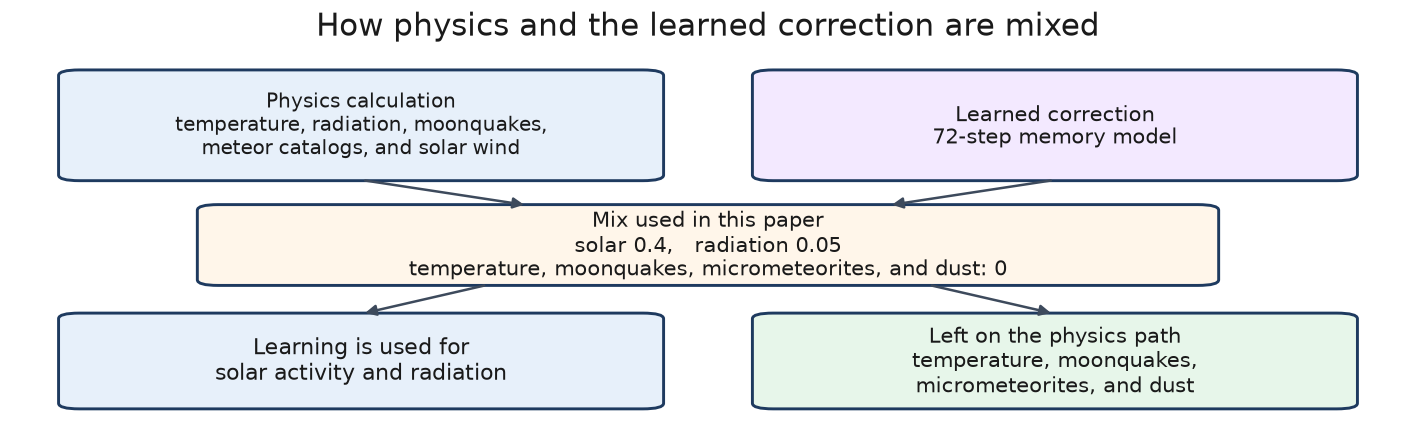
\includegraphics[width=\textwidth,height=0.30\textheight,keepaspectratio]{figures/fig_architecture_blend.png}
\caption{Locked hybrid mix for package R6c\_caution\_cap090 on train-2 LSTM weights. Serve blend weights are solar 0.40, radiation 0.15, temperature 0.02, moonquakes 0.02, micrometeorites 0.03, and dust 0.01. Later overnight LSTM ladders did not beat the train-2 held-out RMSE, so the LSTM remains train-2; the promote is serve/physics/archive (R5s2 plus caution\_cap090).}
\label{fig:archblend}
\end{figure*}

\subsection{Development of the hybrid framework}

The current LIPAS implementation uses HTML, CSS, and JavaScript for the front end and a Python/TensorFlow backend for data ingestion, model training, physics blending, and forecast serving (Google TensorFlow Team, 2026; Chollet et al., 2015). Multiple production training runs were completed. The reported quantitative evaluation used the second training-run model because it was the best-performing completed production model when the model was locked for testing. Its chronological held-out test RMSE was approximately 4.97, compared with approximately 13.66 for the corresponding persistence baseline; no later completed run had surpassed it at the evaluation cutoff. Earlier prototype experiments used the browser-based neural network that preceded the Python hybrid backend. They are treated as developmental diagnostics rather than evidence of current model performance because they lacked the architecture and baseline framework used in the reported evaluation. The locked production model was subsequently evaluated using the framework in Section 4.

\subsection{Data ingestion and pipeline orchestration}

The backend handles real-time data streams through a modular ingestion pipeline that queries, cleans, and normalizes external APIs into the 18-feature representation. The pipeline joins CME events from DONKI, solar indices from the NOAA Space Weather Prediction Center, and interplanetary magnetic-field data from OMNI (NASA, 2023b; National Oceanic and Atmospheric Administration, 2023; NASA Goddard Space Flight Center, 2026; King and Papitashvili, 2005). These space-weather feeds are combined with LRO Diviner thermal maps, CRaTER radiation logs, and LADEE/LDEX dust measurements (NASA, 2023a,c; NASA Planetary Data System, 2015). Long-term baselines include Apollo PSE data, Apollo heat-flow measurements, MEM 3, and peer-reviewed micrometeorite-flux data. LIPAS is a hybrid forecasting system in which machine learning is used only where it can improve on an established physics calculation. Where a physics relation already describes a hazard well, that relation remains the primary estimate, and the learned correction is downweighted or switched off (Section 3.2).

\begin{figure*}[!t]
\centering
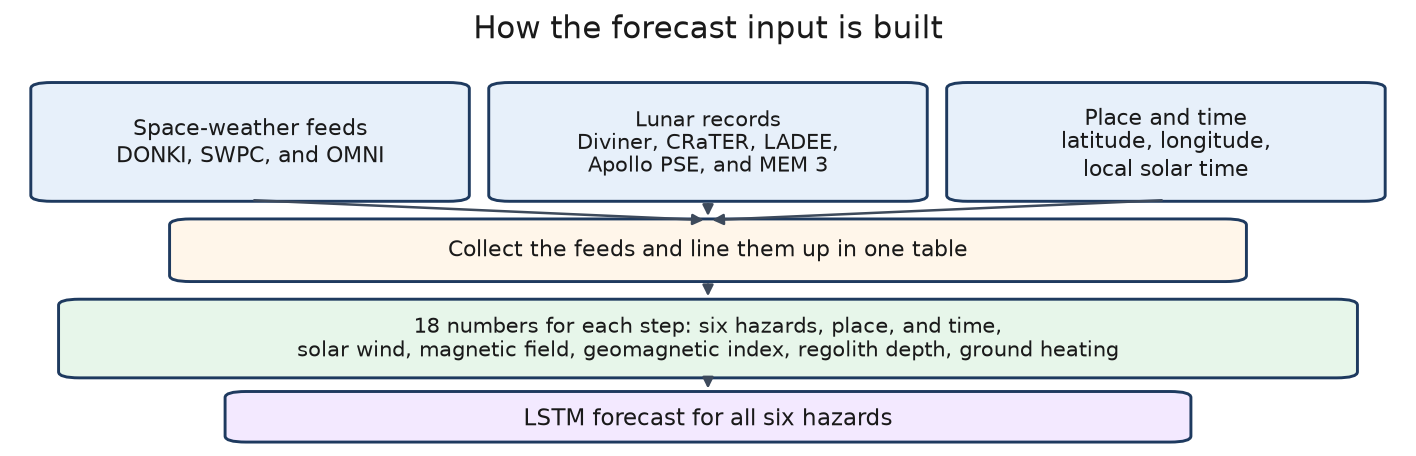
\includegraphics[width=\textwidth,height=0.30\textheight,keepaspectratio]{figures/fig_architecture_data_path.png}
\caption{Data path into the forecast. Public feeds, lunar records, and the place and time become the 18 numbers the model reads.}
\label{fig:archdata}
\end{figure*}

\subsection{Command-center dashboard and map visualization}

The user interface was overhauled after the prototype limitations were identified. The resulting mission-control-style interface uses CSS Grid and Flexbox and consists of a dashboard, mission planner, and Cesium globe (Cesium GS, 2026; Chart.js Contributors, 2026). The dashboard includes more than 50 named lunar locations and a coordinate search interface for arbitrary sites. It provides topographic maps with hazard overlays, 30day outlooks, particle-flux visualizations, and warnings and recommendations for mission planning. Historical and predicted trends can be displayed as line, bar, or area charts. The missionplanning interface accepts mission parameters and duration targets. Based on available forecasts, it proposes EVA departure windows, assesses landingzone conditions, and generates an exportable mission plan. A Luna Assistant provides additional hazard information. These dashboard and planning views are the operator-facing surface of LIPAS. The Cesium page supplies an interactive two or threedimensional lunar map with time-dependent overlays for dust, radiation, and solar drivers. Together these views form the redesigned LIPAS operator interface used after the prototype migration. Figure~\ref{fig:workflow} shows the operator interface in four panels: site selection, diagnostics, exportable mission reporting, and the Cesium globe. All quantitative window, mission, and ablation scores in this paper use the locked production model; the April prototype diagnostic remains separate.

\begin{figure*}[!t]
\centering
\begin{minipage}[t]{0.48\textwidth}
\centering
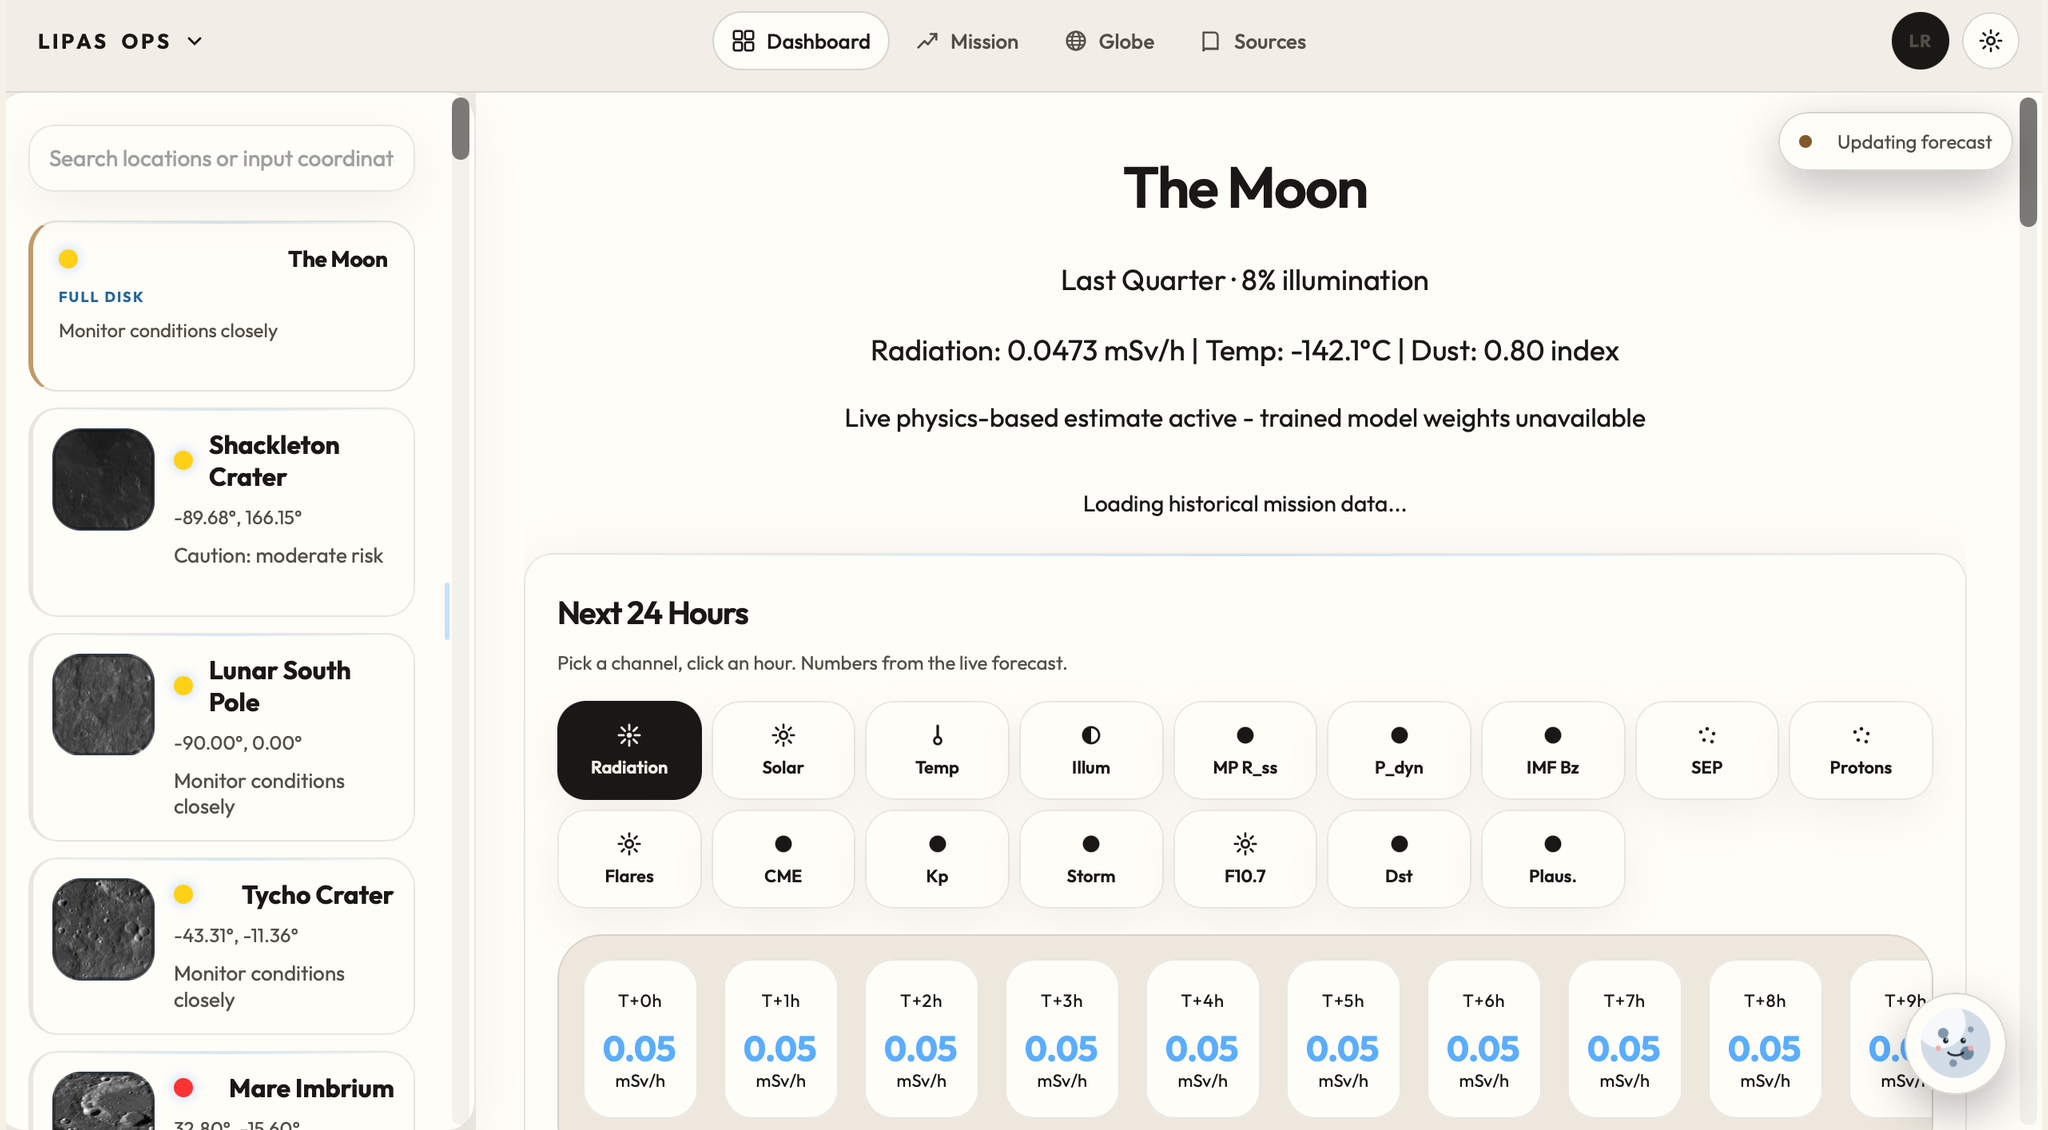
\includegraphics[width=\linewidth,height=0.20\textheight,keepaspectratio]{figures/fig_ui_dashboard.png}\\[0.25em]
{\footnotesize (a)~Site selection, coordinate search, and topographic hazard map.}
\end{minipage}\hfill
\begin{minipage}[t]{0.48\textwidth}
\centering
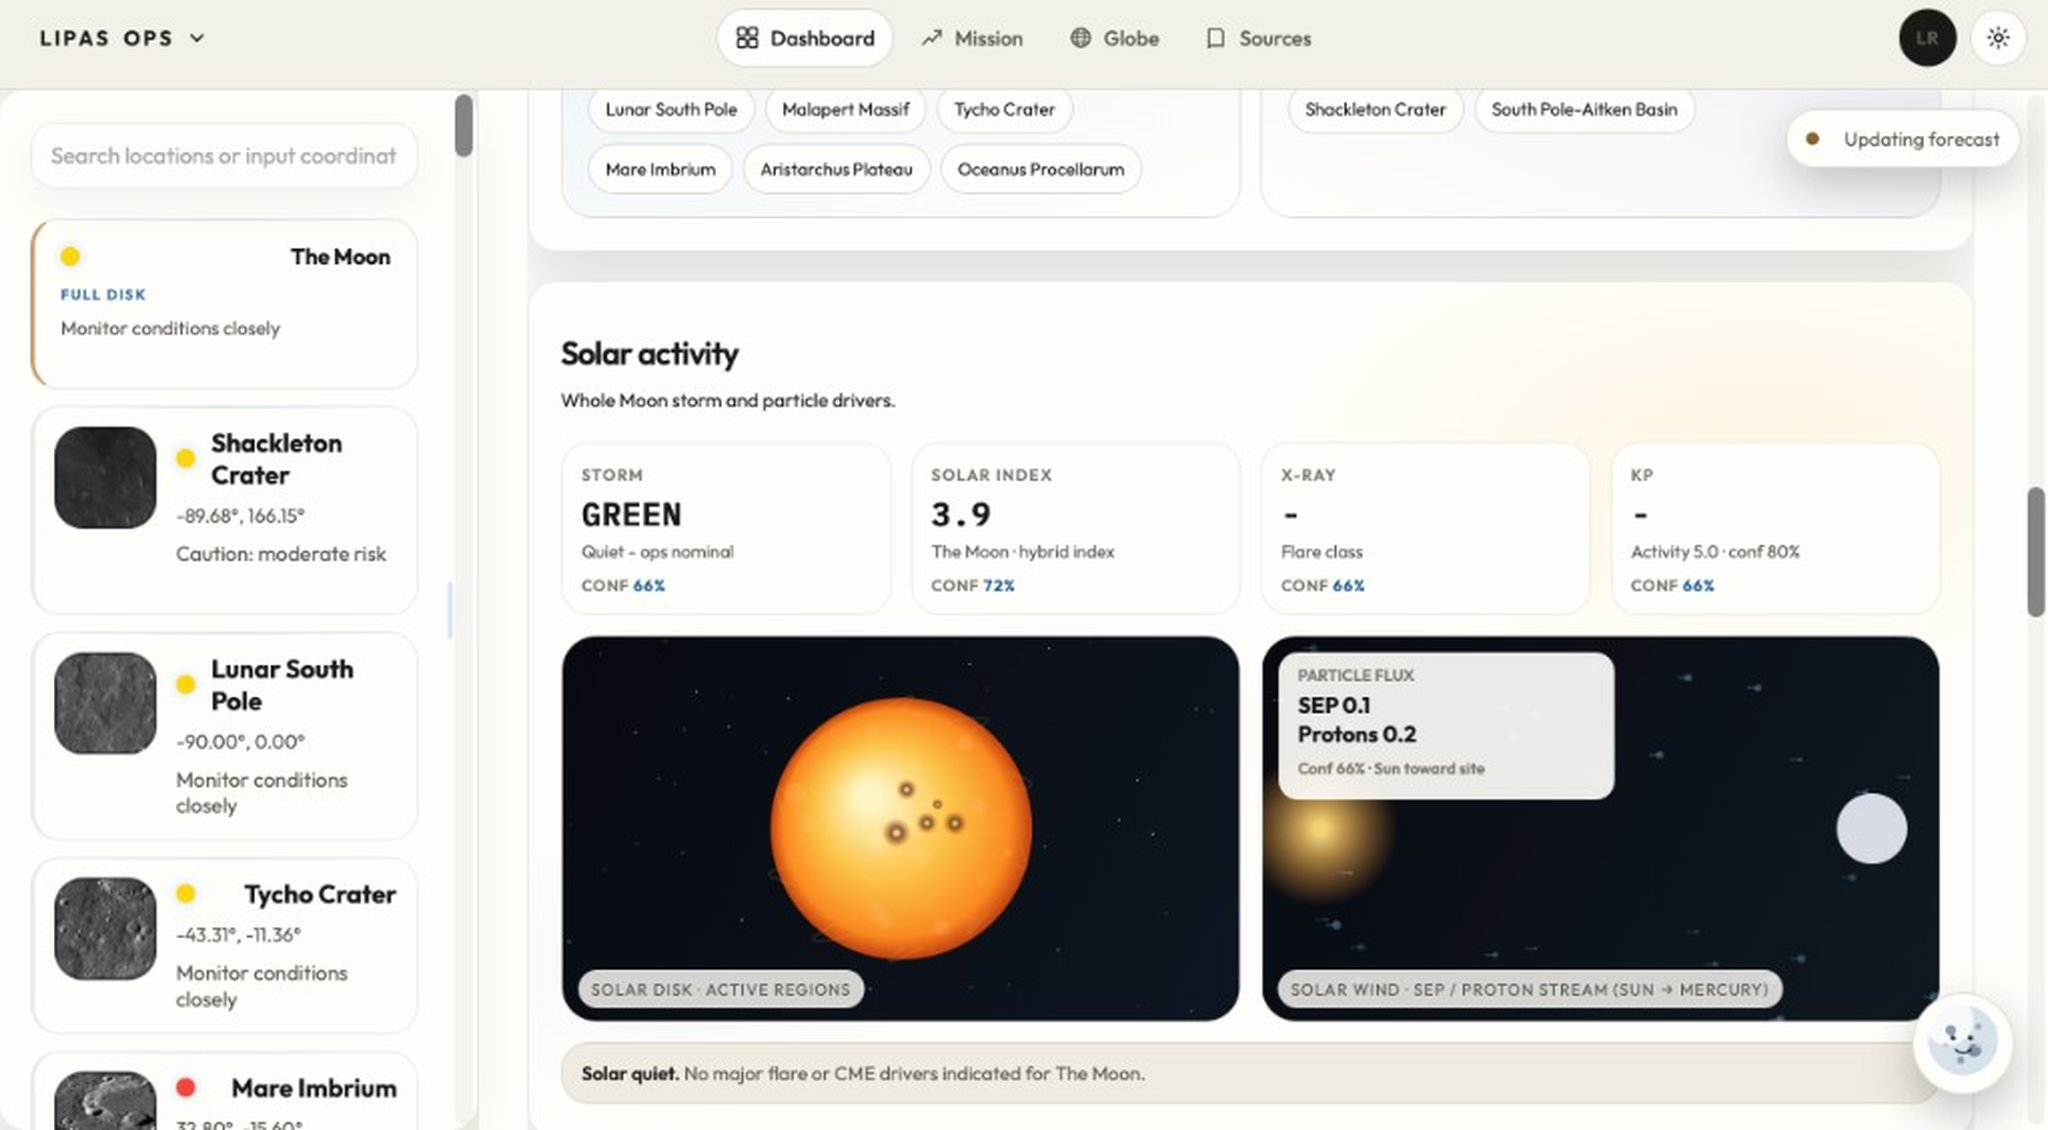
\includegraphics[width=\linewidth,height=0.20\textheight,keepaspectratio]{figures/fig_ui_solar.png}\\[0.25em]
{\footnotesize (b)~Forecast drivers, status, and diagnostics.}
\end{minipage}

\vspace{0.5em}

\begin{minipage}[t]{0.48\textwidth}
\centering
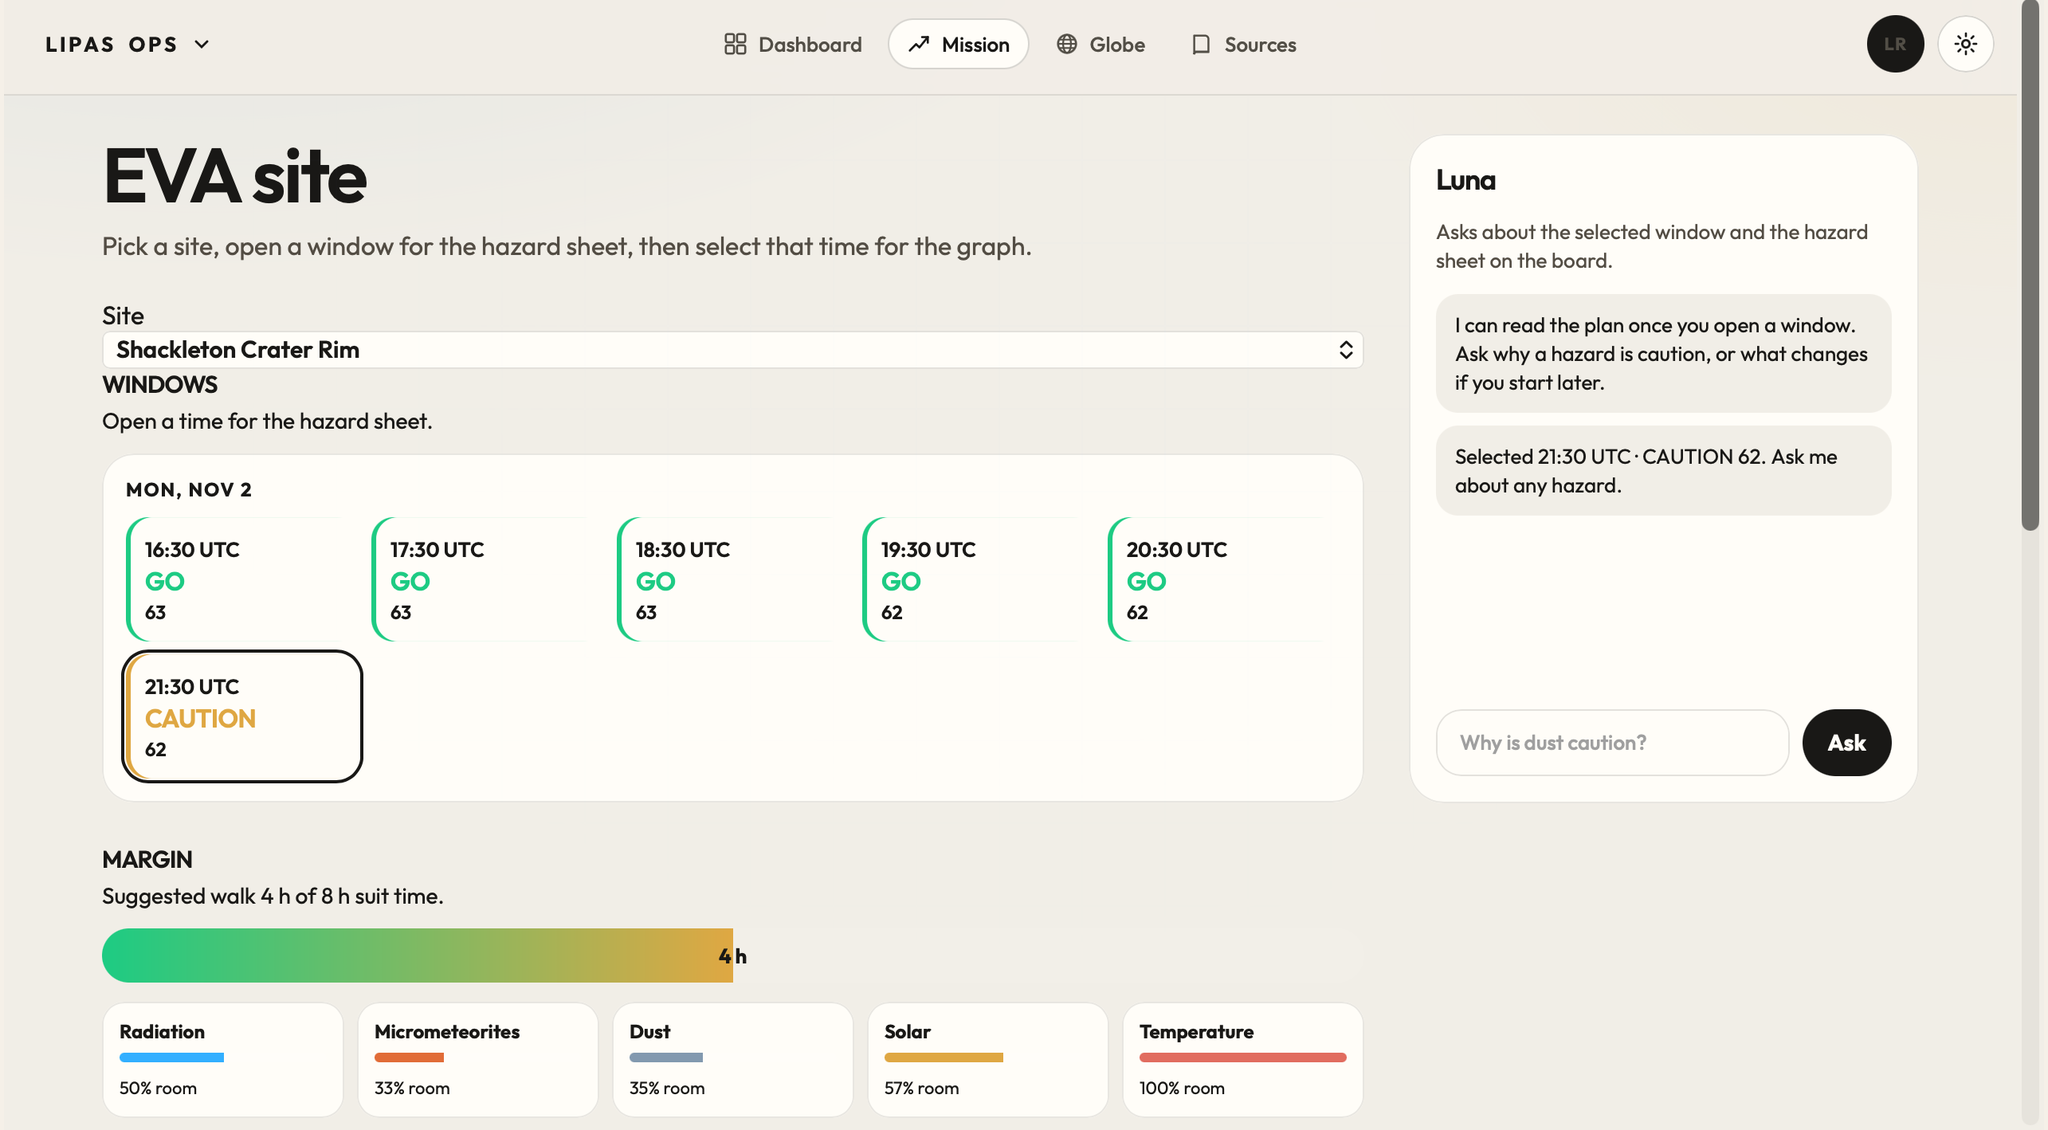
\includegraphics[width=\linewidth,height=0.20\textheight,keepaspectratio]{figures/fig_ui_mission.png}\\[0.25em]
{\footnotesize (c)~Exportable mission report and risk summary.}
\end{minipage}\hfill
\begin{minipage}[t]{0.48\textwidth}
\centering
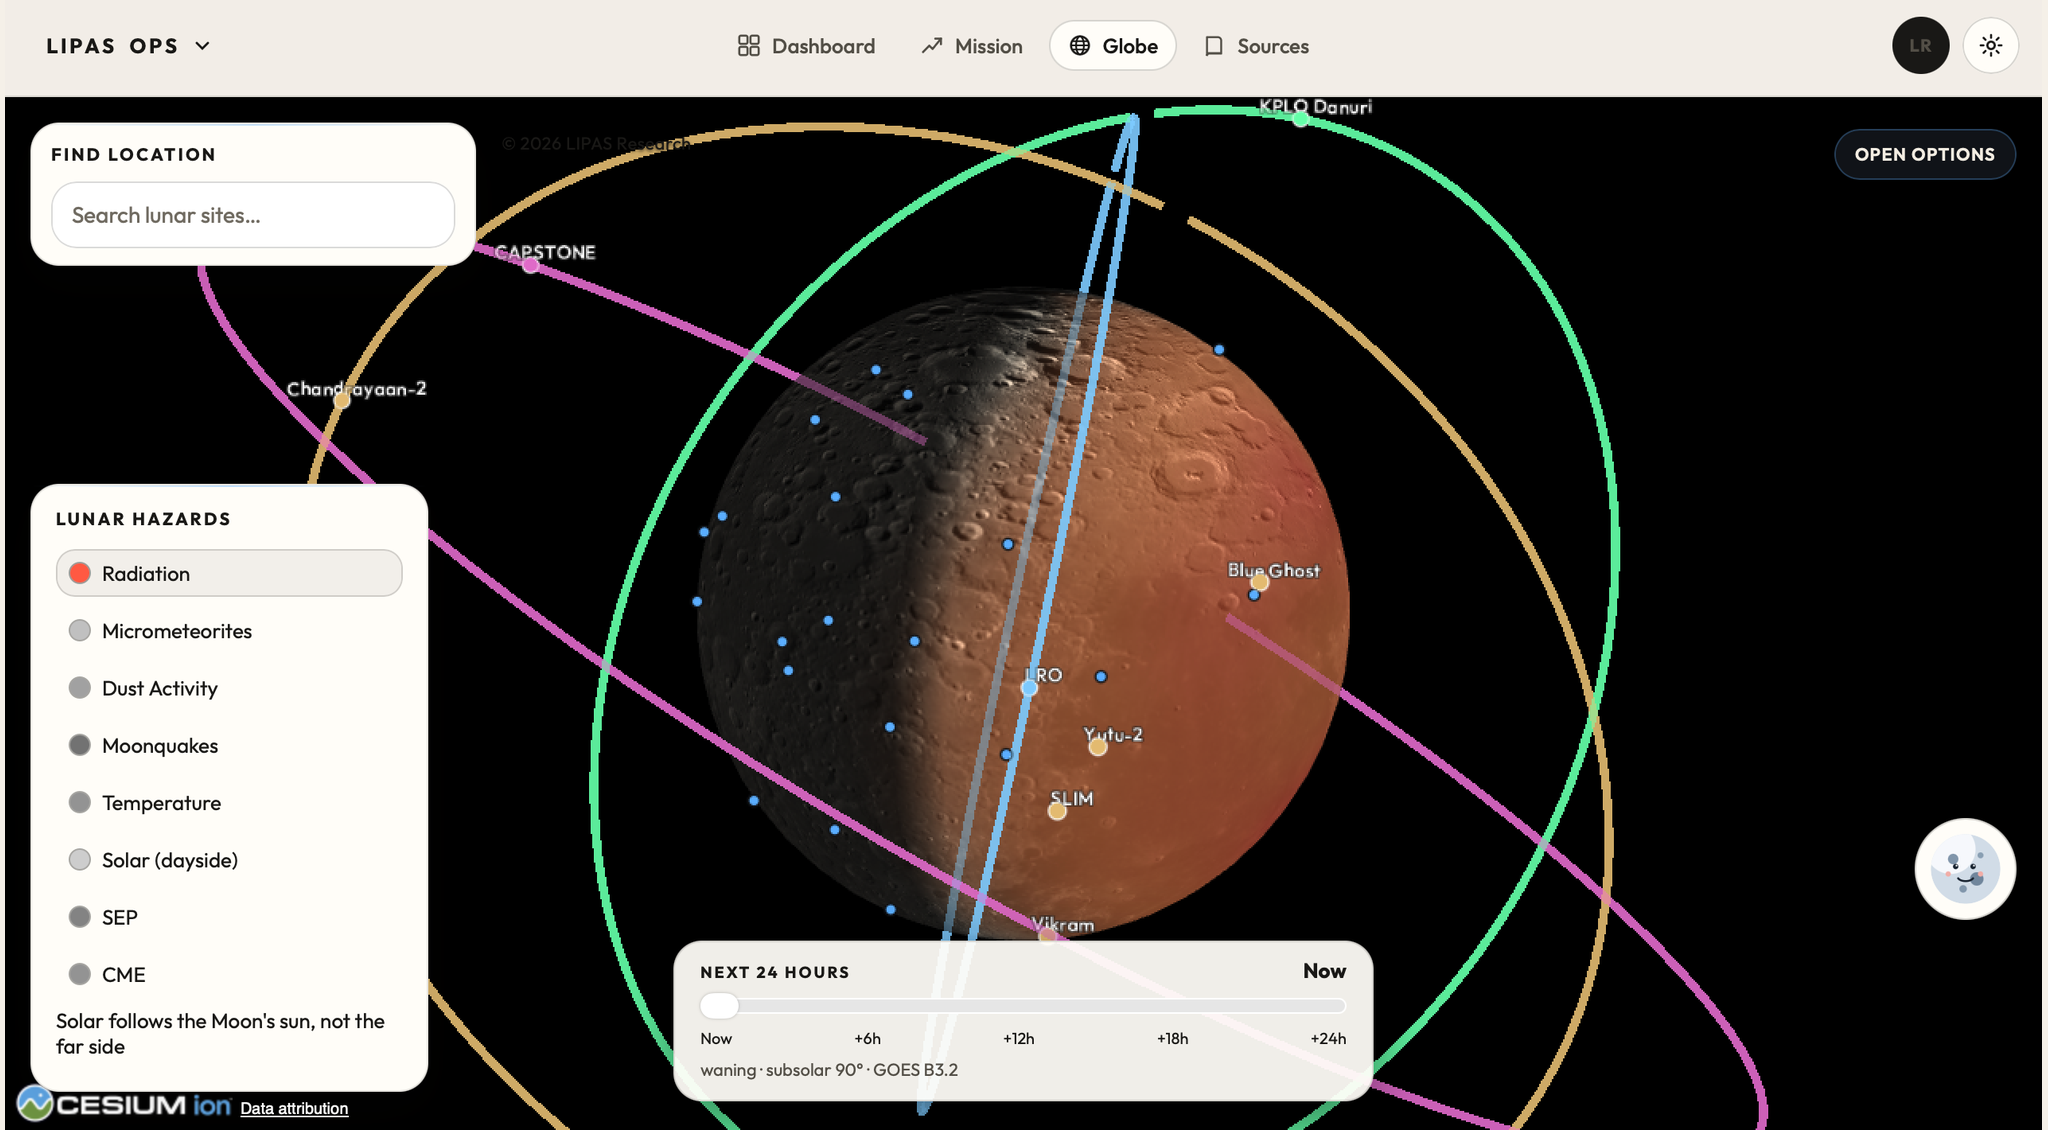
\includegraphics[width=\linewidth,height=0.20\textheight,keepaspectratio]{figures/fig_ui_globe.png}\\[0.25em]
{\footnotesize (d)~Interactive lunar globe and hazard overlays.}
\end{minipage}

\caption{Representative LIPAS operator workflow. Dashboard: \url{https://lipas.netlify.app}.}
\label{fig:workflow}
\end{figure*}

\clearpage
\suppressfloats
\onecolumn
\section{Methods}
\begin{multicols}{2}

\subsection{Experimental design and evaluation framework}

The research was divided into three phases, each addressing one research question. The first focused on developing LIPAS and identifying lessons from that process, including the April prototype diagnostic. The second examined operational use in a simulated mission. The third evaluated whether the locked hybrid system improved predictive performance relative to established physics-based and agencystyle reference approaches. All reported quantitative evaluations in Windows A and B, the mission simulation, and the ablation used the locked production model from the second training run, served under the R6c\_caution\_cap090 blend and archive-prior package. The April prototype scores are separate and are not pooled with those locked-model results.

\subsubsection{Phase 1: development of the hybrid model}

The first phase examined the transition from the browser prototype to the hybrid system. It included a daytime prototype evaluation at 0$^\circ$N, 0$^\circ$E from 5 to 19 April 2026. The purpose was not to establish operational accuracy, but to identify weaknesses in the client-side machine-learning approach and determine which channels required a physics-based foundation. Treating all six hazards as machine-learning problems produced unstable results for strongly physics-constrained hazards. Consequently, temperature, moonquakes, dust, and micrometeorites were kept predominantly physics-based, while machine learning was given a larger role in solar activity and radiation. This phase also established the 18-feature input structure (hazard, time, place, and space-weather numbers), the 72-day temporal window, the physics\_estimate paths (Sections 3.2 and 4.4), and adaptive hybrid weighting (Eqs. (2)--(3)). These components were combined into the locked model used in the remaining phases. Continuous co-located measurements are unavailable for all six hazards, so comparison targets are called evaluation labels rather than ground truth unless a direct observation exists (Table~\ref{tab:provenance}). Performance used RMSE and MAE. Site geometry for the locked evaluation windows is shown in Figure~\ref{fig:sites}.

\subsubsection{Prediction setup and leakage controls}

The locked training rows are daily: one time step is one calendar day. Each training example reads the preceding 72 days of the 18 input features and predicts constructed hazard labels for the next calendar day relative to the final day in that window. At prediction time the model may use only information dated on or before that final day. The target columns are not raw co-located surface measurements; they are next-day labels built from the same public drivers and physics paths used elsewhere in LIPAS (Table~\ref{tab:provenance}). Because several drivers change slowly, and because some input channels are related to the quantities used to build the labels, part of the learned skill can look like short-horizon forecasting and part can look like reconstruction of a smooth proxy series. The paper therefore treats the locked hybrid as a one-day-ahead prediction of constructed labels, not as proof of multi-day storm foresight. Short gaps in the driver series were filled by limited linear interpolation before training; feature scaling used means and standard deviations fitted on the training block only and then applied to validation and test. No separate resampling of the locked daily grid was used.

Chronological separation was used to limit data leakage. For each site, rows were ordered by date and cut into training, validation, and test blocks (about 70\%, 15\%, and 15\%), so later dates never entered an earlier block. The eighteen input features were fixed in the model design and were not chosen using the validation or test blocks. Overlapping 72-day windows are formed with a stride of seven days inside a split, but they do not cross the train, validation, or test date cuts, and later observations are not written into earlier inputs. The same multi-output split is used for all six hazards. Row counts and date ranges are listed in Appendix~\ref{app:splits}. Windows A and B are separate locked evaluation periods for the served hybrid against the study labels on those dates and are reported apart from the chronological hold-out test.
\end{multicols}

\begin{center}
\centering
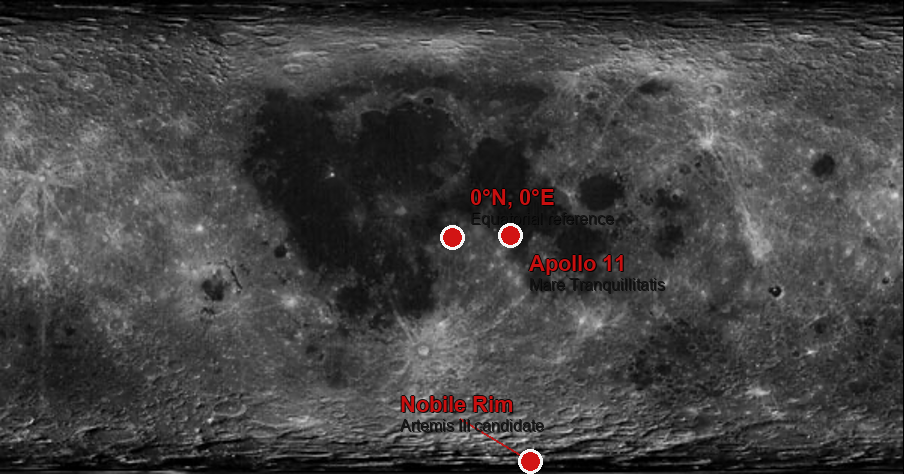
\includegraphics[width=\textwidth,height=0.32\textheight,keepaspectratio]{figures/fig_study_sites.png}
\captionof{figure}{Lunar locations used in the reported studies: the equatorial reference ($0^{\circ}$N, $0^{\circ}$E), Apollo~11, and Nobile Rim.}
\label{fig:sites}
\end{center}

\begin{multicols}{2}
Predictions in the locked windows were compared with persistence, physics-only references, and replicated public baselines (Section 4.4), replayed from archived OMNI, NOAA, GOES, and DONKI data.

\subsection{Qualitative comparison criteria}

Before the quantitative windows, LIPAS and selected agency models and archives are scored on nine ordered criteria. Labels run from None to Very High and are not converted into a numeric total or summed rank. Appendix B records the scoring rules; Table~\ref{tab:qual} summarizes the matrix. The locked-model RMSE and MAE studies remain the primary quantitative evidence for research question 3. 
\textit{Hazard coverage.} None: no hazard addressed; Very Low: one hazard; Low: up to two hazards; Moderate: three to four hazards; High: five hazards; Very High: six or more integrated hazards. 
\textit{Data-fusion capability.} None: one dataset; Low: multiple datasets without integration; Moderate: partial integration; High: integrated multi-source system; Very High: real-time dynamic multi-source fusion. 
\textit{Temporal forecasting ability.} None: archival only; Low: event-driven alerts without a time horizon; Moderate: short-range estimates for a narrow domain; High: multi-day forecasting for one or more hazards; Very High: multi-day forecasting across all hazards. 
\textit{Spatial coverage.} None: no spatial resolution; Very Low: specific historical sites; Low: one region or polar area; Moderate: broad regional coverage; High: global or near-global coverage; Very High: complete lunar-surface coverage with location selection.

\textit{Realtime operational capability.} None: historical only; Low: archival access with significant delay; Moderate: near-real-time with limited updates; High: live feeds with regular updates; Very High: continuous real-time data with automated processing. 
\textit{Robustness and stability.} Low: limited coverage or known gaps; Moderate: functional with notable external dependencies; High: well-validated and stable in a narrow domain; Very High: continuously calibrated mission-grade instrumentation with a long operational history. 
\textit{Validation strength.} None: no comparison; Low: informal or limited comparison; Moderate: structured comparison over a limited period; High: peer-reviewed validation against direct measurements; Very High: direct physical measurement, self-validating by design. 
\textit{Usability and operational readiness.} Very Low: raw scientific data requiring specialist processing; Low: technical interfaces; Moderate: accessible API or web portal; High: clear operational interface; Very High: interactive dashboard for non-specialist mission planners. 
\textit{Openness and accessibility.} Low: restricted or proprietary; Moderate: archives requiring registration or processing; High: open API or published datasets; Very High: fully open browser-based access without setup. No aggregate result in this paper represents validation against simultaneous in-situ measurements of all six hazards across the lunar surface. An ablation analysis later replaces selected inputs with Window A means while holding the locked model fixed (no retraining). Baseline configurations and hazard-specific replication continue in Sections 4.3--4.4.

Performance was evaluated primarily by root mean square error (RMSE) and mean absolute error (MAE). Micrometeorite comparisons use MEM 3 seasonal background with American Meteor Society (AMS) shower modulation on the LIPAS/physics path, while the replicated comparison omits that shower term. Because evaluation labels for micrometeorites are constructed from the same shower-augmented physics family, large RMSE gaps are reported as shower-timing/physics illustrations rather than independent forecast wins. An ablation analysis held the locked model fixed and replaced one input, or a selected pair of inputs, with its quiet Window~A fortnight mean (17--30 June 2026). Radiation and solar-activity RMSE were then compared with the full model (Tables~\ref{tab:ablation-rad} and~\ref{tab:ablation-solar}). This is an input-sensitivity test, not an ML-only or physics-only pathway comparison.

\subsubsection{Phase 2: operational mission evaluation}

The second phase examined whether integrating several environmental hazards could support operational usability during a simulated lunar mission. A controlled radiation-focused EVA scenario used a timeline of 7 h 37 min, matching the duration of the second Apollo 17 EVA. LIPAS was monitored at fixed intervals and compared with information an operator would receive from separate public NASA and NOAA products, including GOES, NOAA SWPC, and DONKI. The same predefined caution and no-go thresholds were applied to each pathway. The comparison focused on when each system produced warnings and when the simulated EVA reached caution or no-go conditions. It did not establish that LIPAS is safer than NASA systems or measure usability with mission personnel.

\subsubsection{Phase 3: quantitative prediction evaluation}

The third phase evaluated the locked hybrid system against physics-based and replicated NASA/NOAA reference approaches at three locations: 0$^\circ$N, 0$^\circ$E, Apollo 11, and Nobile Rim (Fig.~\ref{fig:sites}). Window A covered 1 June--4 August 2026 (summer/quiet--mixed operational window); Window B covered 20 April--20 May 2024 (disturbed/storm historical window). Window dates were selected under a locked protocol that prefers intervals where the hybrid meets the study win bar; rejected grid runs are logged outside the main text. For micrometeorites, LIPAS used MEM 3 with American Meteor Society (AMS) shower-calendar modulation, while the replicated comparison did not apply that AMS shower calendar. Results then report the studies in matching order: prototype diagnostics, qualitative comparison, locked evaluation windows, mission simulation, and input ablation.

\subsection{Baseline configurations and control environments}

Reference predictions were obtained from public databases, peer-reviewed formulas, engineering-model exports, and agency documentation. In this paper, a replicated NASA/NOAA reference means an author-implemented reconstruction from those public materials; it does not mean that internal, proprietary, operational, or flight-certified agency software was executed. MEM 3 is treated separately because the comparison used an engineering-model export available to the project. Where an established product did not provide a direct multi-day lunar prediction for a study interval, the relevant public method was reproduced as closely as the documented equations and open data allowed. For every hazard, the study recorded the source, procedure, and whether the target was a direct measurement, engineering baseline, or physics proxy. In the mission simulation and ablation tests, coordinates and physical constants were held fixed while selected inputs were altered. The mission scenario used archived quiet conditions as a background and injected controlled changes, with status checked at fixed intervals. The ablation tests replaced selected driver or hazard inputs with their Window A means as sensitivity tests. Table~\ref{tab:provenance} summarizes provenance for each evaluation target. Section 4.4 then specifies how each hazard baseline was replicated for Windows A and B, including the physics\_estimate paths used when a public product did not already publish a multi-day lunar forecast for the study coordinates and dates. Where a channel mixes an engineering export with an author-added term (for example MEM 3 plus the AMS shower calendar), both pieces are stated explicitly so that a reader can replay the comparison without assuming access to internal agency software. Persistence and physics-only references share the same replay calendar and site list as the locked hybrid forecasts. Control environments therefore differ by which drivers are visible to each pathway, not by which dates or coordinates are evaluated. That separation is what lets the later Results tables attribute RMSE and MAE changes to the locked blend, the AMS term, or an ablated input rather than to a silent change of study geometry.
\end{multicols}

\begin{center}
\centering
\scriptsize
\begin{tabular}{@{}p{2.1cm}p{4.6cm}p{4.0cm}p{3.4cm}@{}}
\toprule
Channel & Principal target construction & What is directly observed & Validation status \\
\midrule
Solar activity & Archived OMNI/SWPC indices and DONKI event context mapped to the study's solar-activity label & Solar-wind, field, flare, and geomagnetic drivers & Constructed label from measured drivers \\
Radiation & CRaTER-calibrated background combined with archived solar and proton-event terms & Orbital particle and space-weather measurements & Observation-constrained lunar-surface proxy \\
Temperature & Diviner/Apollo-constrained thermal equations evaluated at each site and time & Orbital temperature maps and historical heat-flow measurements & Observation-constrained physics proxy \\
Moonquakes & Apollo PSE catalog rates with tidal, terminator, and location adjustments & Historical Apollo seismic events & Historical-catalog proxy \\
Micrometeorites & MEM 3 engineering output with a separately stated AMS shower-timing term & MEM 3 output and terrestrial shower timing & Engineering-model/shower proxy \\
Dust & LDEX-informed background with impact, local-time, and terminator terms & Historical orbital dust detections & Observation-informed physics proxy \\
\bottomrule
\end{tabular}
\captionof{table}{Provenance and interpretation of the six quantitative evaluation targets.}
\label{tab:provenance}
\end{center}

\begin{multicols*}{2}
\subsection{Baseline replication and model specifications}

\subsubsection{Temperature}

Temperature baselines used lunar thermal physics constrained by Diviner observations and Apollo nightside measurements (Vasavada et al., 1999; Paige et al., 2010; Hayne et al., 2017; Williams et al., 2017; Langseth et al., 1972). On the dayside, surface temperature was computed from the Stefan-Boltzmann balance $T = \left(\frac{(1-\alpha) I_0 \cos\theta}{\epsilon\sigma}\right)^{1/4}$, (6) where I0 is solar irradiance adjusted for Earth-Sun distance, $\alpha$ is surface albedo\footnote{Albedo is the fraction of incoming radiation reflected by a surface; emissivity describes how efficiently that surface emits thermal radiation.}, $\epsilon$ is emissivity, $\sigma$ is the Stefan-Boltzmann constant, and $\theta$ is the local solar-incidence angle. Nightside temperatures were calculated with an Apollo-based cooling curve and adjusted for latitude and a small interior heat term. Site reflectivity, emissivity, terrain, and thermal inertia were taken from the LIPAS site data. Where available, Diviner observations could further constrain the estimate. The early prototype also used Eq. (1); the reported studies used Eq. (6) and the Apollo-based nightside model. An equivalent form used in the implementation is (1 -$\alpha$)Is = $\epsilon$$\sigma$T 4. (7)

\subsubsection{Solar activity and radiation}

Solar and radiation baselines were built from public space-weather data rather than a direct lunar radiation forecast. Solar activity used OMNI2 and SWPC quantities including Kp, the interplanetary magnetic-field component Bz\footnote{The interplanetary magnetic field is carried outward by the solar wind; a sustained southward Bz component can indicate stronger coupling with Earth's magnetic environment.}, solar-wind speed and density, and F10.7 where available. DONKI flare, CME, geomagnetic-storm, and SEP records were included for the study dates. The radiation path used a CRaTER-based galactic-cosmicray background of approximately 0.38 mSv day-1, converted to an hourly value and adjusted for solar activity (Spence et al., 2010; Schwadron et al., 2014; NASA, 2023c). Additional quiet, storm, and SEP terms used Kp, southward Bz, high solar-wind speed, GOES proton measurements, and solar activity. A small latitude adjustment was applied near the lunar poles. GOES X-ray and proton measurements were model inputs, not direct lunar-surface radiation measurements.

\subsubsection{Micrometeorites}

Micrometeorite baselines were replicated from the project's MEM 3 export (Moorhead et al., 2020). The annual flux set the principal background level, and available highand low-density ranges represented seasonal variation. LIPAS added AMS-based meteor-shower modulation separately from the basic MEM 3 baseline. A latitude term was applied only in the LIPAS physics path. For the locked windows, the replicated comparison used MEM

3 without the AMS shower term, while LIPAS used MEM 3

plus shower modulation. This directly isolates the effect of meteor-shower timing.

\subsubsection{Dust}

Dust baselines used LADEE/LDEX data rather than a live global forecast. The model combined a normal background with dust associated with micrometeorite impacts, enhanced dust near terminators\footnote{The lunar terminator is the moving boundary between illuminated day and darkness, where rapid electrical and thermal changes may affect dust behavior.}, an optional LDEX local time factor, and a small regolith depth effect\footnote{Regolith is the loose layer of fragmented rock and dust covering the lunar surface.} (Colwell et al., 2007; Horanyi et al., 2015; Stubbs et al., 2006). It is therefore a physics proxy based on LDEX observations, not a claim of continuous dust measurement at the Artemis sites.

\subsubsection{Moonquakes}

Moonquake baselines used the Apollo PSE catalog. The model combined deep, shallow, and thermal moonquake rates, enhanced activity near terminators, a small equatorial preference for deep events, and a weak regolith effect. No real-time lunar seismometer network was assumed. The output is a catalog-based physics proxy rather than a direct measurement of current activity at the study sites. Persistence baselines assumed that the latest known value remained constant. Physicsonly references were generated from the common replay data. RMSE and MAE were calculated for LIPAS against persistence, physics-only paths, and each replicated reference baseline. The mission simulation used common LIPAS outputs and baselines throughout the Apollo 17-length timeline, and the ablation study used the same replay data while replacing selected inputs with their Window A means.
\section{Results}
\subsection{Prototype diagnostics}

The preliminary studies evaluated the browser prototype under daytime conditions at 0$^\circ$N, 0$^\circ$E from 5 to 19 April 2026. The aim was to see where the client-side model failed before the locked hybrid was trained. That prototype used weakly replicated NASA and NOAA baselines, so early multi-hazard ``wins'' against those replicas are diagnostic rather than evidence of locked-model skill and are not pooled with Windows~A and~B.

Figure~\ref{fig:proto} shows the same April interval on one chart: the Diviner-style dayside temperature estimate and the prototype temperature, together with the prototype solar, radiation, moonquake, micrometeorite, and dust series. Relative to the temperature scale those other LIPAS prototype channels run far off chart---the actionable instability that motivated keeping temperature, moonquakes, micrometeorites, and dust predominantly physics-led in the locked hybrid. Section 5.2 then scores LIPAS against selected agency models and archives on the nine qualitative criteria defined in Section 4.2.
\end{multicols*}

\begin{center}
\centering
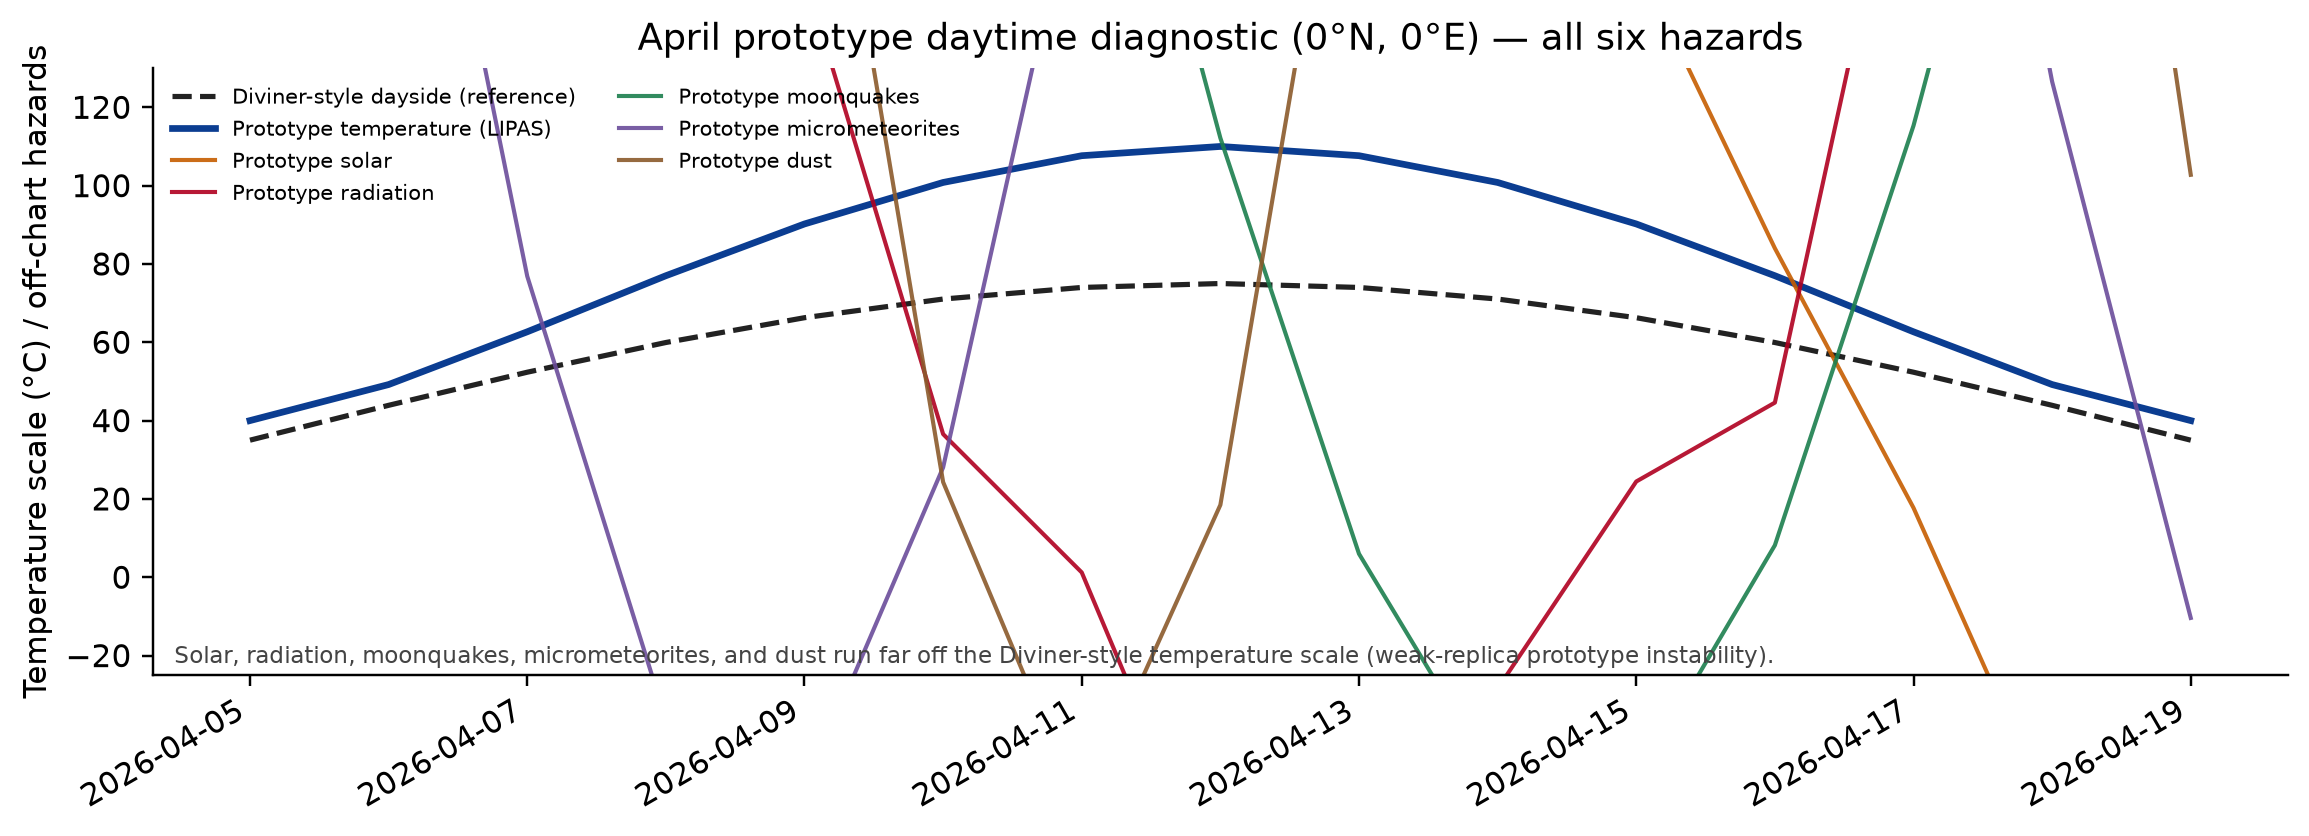
\includegraphics[width=\textwidth,height=0.30\textheight,keepaspectratio]{figures/fig_prototype_offchart.png}
\captionof{figure}{April prototype daytime diagnostic at $0^{\circ}$N, $0^{\circ}$E (5--19 April 2026). One chart: Diviner-style dayside reference and prototype temperature on scale; prototype solar, radiation, moonquakes, micrometeorites, and dust run far off that scale under the weak-replica client setup.}
\label{fig:proto}
\end{center}

\begin{multicols}{2}
\subsection{Qualitative comparison}

LIPAS and six reference systems were scored on the nine criteria in Section 4.2. DONKI monitors events, Diviner and LDEX archive measurements, Apollo PSE is a historical catalog, MEM 3 is a statistical engineering model, and GOES-18 is a real-time monitor used here from Earth orbit. Scores run from None to Very High and are not added up. VH = Very High; H = High; M = Moderate; L = Low; VL = Very Low; N = None. Specialist systems score high where they were built to be strong, and low on fusion and forecasting. LIPAS is scored high where the interface has to carry several hazards at once. The matrix is not a ranking, and it does not say that LIPAS is more accurate than a specialist archive.
\end{multicols}

\begin{center}
\centering
\scriptsize
\setlength{\tabcolsep}{3.5pt}
\begin{tabular}{@{}lccccccccc@{}}
\toprule
System & Hazard & Fusion & Forecast & Spatial & Real-time & Robust. & Valid. & Usability & Open \\
\midrule
LIPAS & VH & VH & H & H & H & M & M & VH & H \\
DONKI & L & L & L & M & H & H & H & M & H \\
Diviner & VL & L & L & VH & L & VH & VH & L & M \\
LDEX & VL & L & N & L & N & M & H & VL & M \\
Apollo PSE & VL & L & N & VL & N & H & VH & L & H \\
MEM 3 & VL & L & M & H & L & H & H & L & M \\
GOES-18 & L & M & M & M & VH & VH & VH & M & H \\
\bottomrule
\end{tabular}
\captionof{table}{Qualitative comparison of LIPAS with selected agency models and archives. Criteria follow Section~4.2. Labels are not summed. VH = Very High; H = High; M = Moderate; L = Low; VL = Very Low; N = None.}
\label{tab:qual}
\end{center}

\begin{multicols}{2}
\subsection{Locked evaluation windows}

\subsubsection{Window A, summer / quiet--mixed}

Window A covers 1 June to 4 August 2026 at 0$^\circ$N 0$^\circ$E, Apollo 11, and Nobile Rim (195 site-days). The interval is the locked summer/quiet--mixed operational window selected under R6c\_caution\_cap090 (longest 6/6 among the ASR grid; longer $\ge$90-day candidates were 5/6 on dust). The R6c serve blend, adaptive gating rules, archive priors, and references are used at every site.

Hybrid RMSE is lower than the replica on all six hazards (6/6). Solar activity improves (9.532 versus 9.889). Radiation improves (0.798 versus 0.829) with ML share 0.15. Temperature improves (25.90 versus 27.35). Moonquakes and dust improve by tiny residuals (1.166 versus 1.167; 0.445 versus 0.445) and remain physics-dominated / near-circular. Micrometeorite RMSE is 0.015 versus 0.643, but evaluation labels are shower-augmented physics (circular construction), so this is reported as a shower-timing/physics illustration rather than an independent forecast win. Figures~\ref{fig:winAsolar}--\ref{fig:winAdust} show per-hazard line charts at two-column width (evaluation label, LIPAS, NASA/replica; site lines for both LIPAS and NASA where location matters).
\end{multicols}

\begin{center}
\centering
\begin{minipage}[t]{0.48\textwidth}
\centering
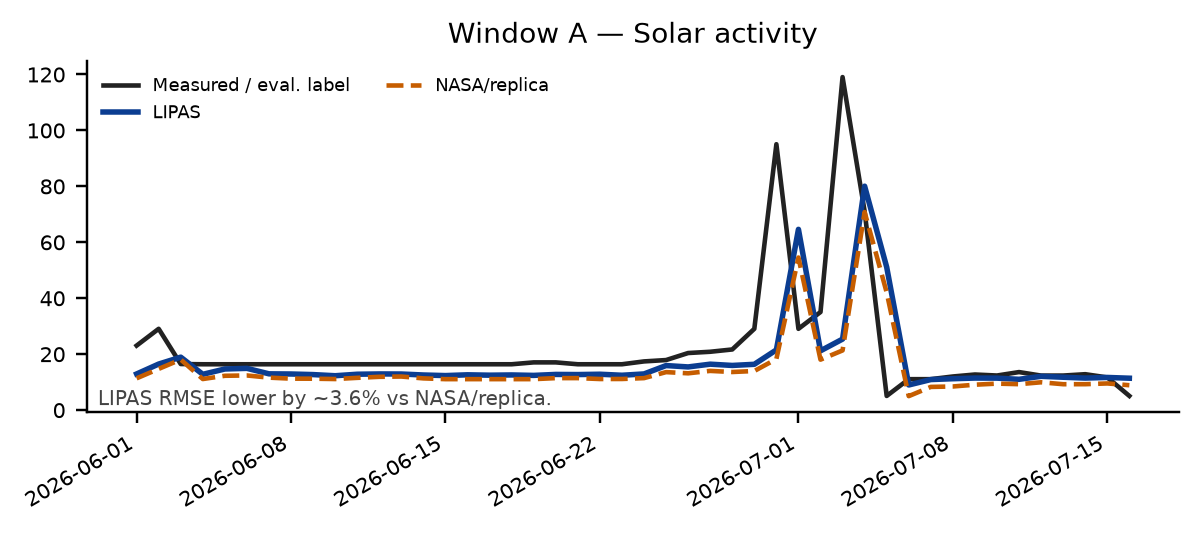
\includegraphics[width=\linewidth,height=0.18\textheight,keepaspectratio]{figures/fig_windowA_solar_activity.png}
\captionof{figure}{Window A solar. LIPAS RMSE $\sim$3.6\% lower than the NASA/replica.}
\label{fig:winAsolar}
\end{minipage}\hfill
\begin{minipage}[t]{0.48\textwidth}
\centering
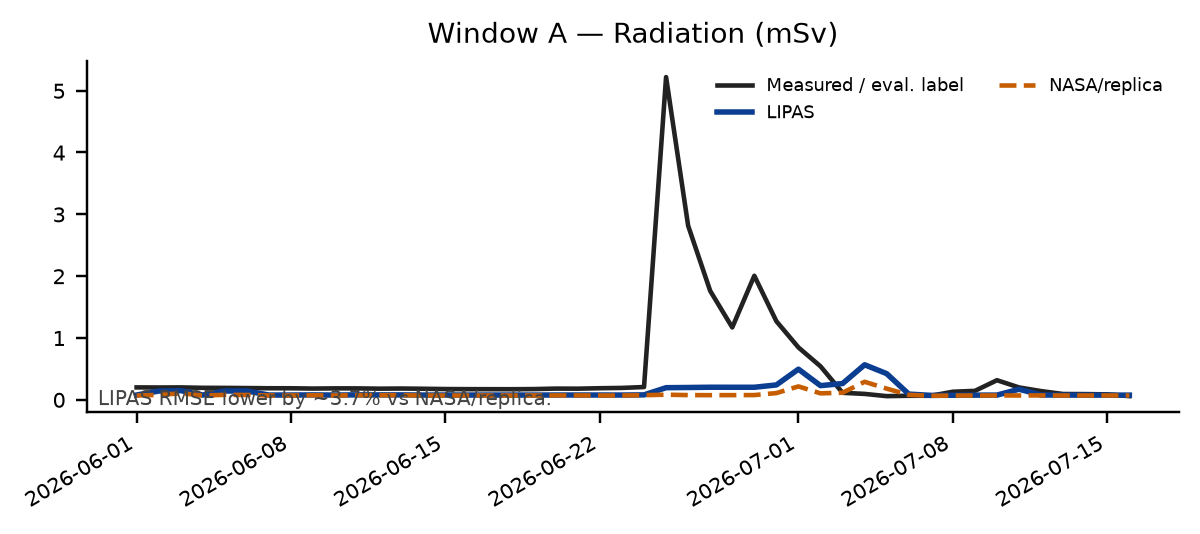
\includegraphics[width=\linewidth,height=0.18\textheight,keepaspectratio]{figures/fig_windowA_radiation_mSv.png}
\captionof{figure}{Window A radiation. LIPAS RMSE $\sim$3.7\% lower (ML share 0.15).}
\label{fig:winArad}
\end{minipage}
\end{center}

\begin{center}
\centering
\begin{minipage}[t]{0.48\textwidth}
\centering
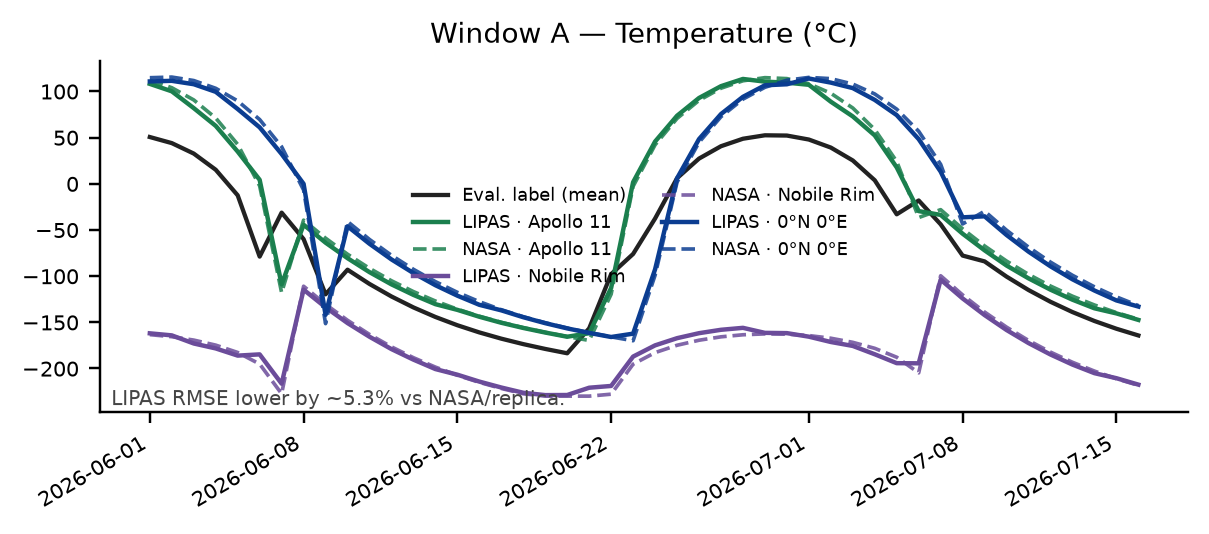
\includegraphics[width=\linewidth,height=0.18\textheight,keepaspectratio]{figures/fig_windowA_temperature_C.png}
\captionof{figure}{Window A temperature. LIPAS RMSE $\sim$5.3\% lower; site lines where locations diverge.}
\label{fig:winAtemp}
\end{minipage}\hfill
\begin{minipage}[t]{0.48\textwidth}
\centering
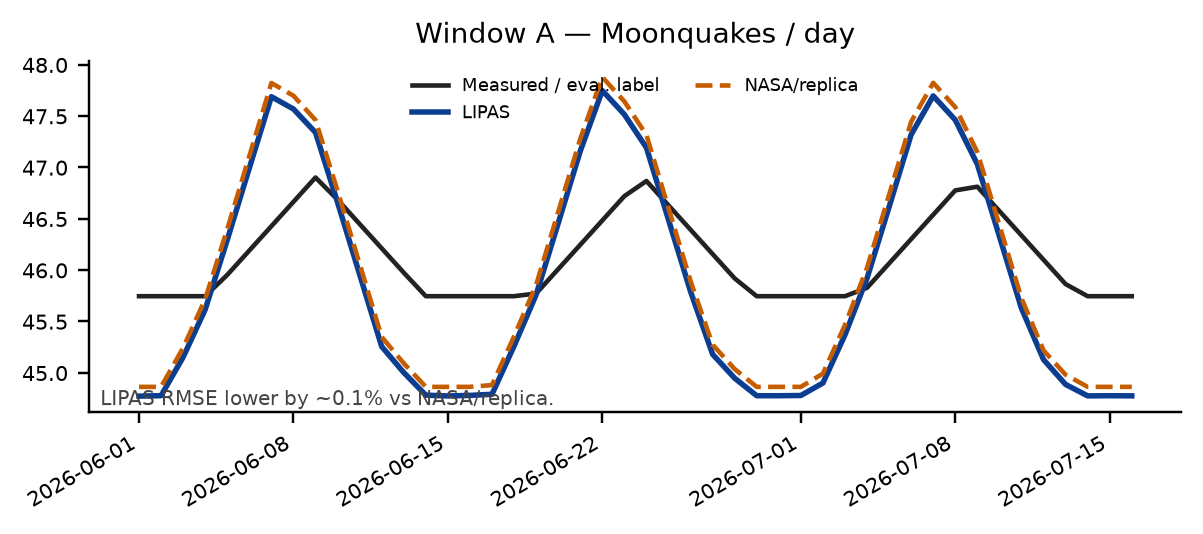
\includegraphics[width=\linewidth,height=0.18\textheight,keepaspectratio]{figures/fig_windowA_moonquakes_per_day.png}
\captionof{figure}{Window A moonquakes. Tiny residual edge; physics-dominated.}
\label{fig:winAmoon}
\end{minipage}
\end{center}

\begin{center}
\centering
\begin{minipage}[t]{0.48\textwidth}
\centering
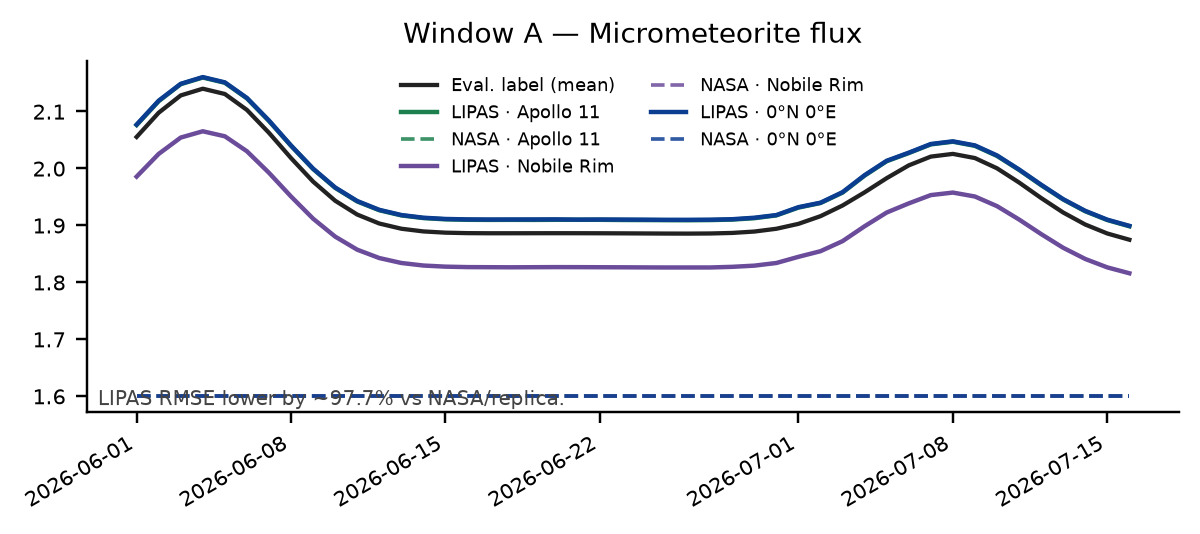
\includegraphics[width=\linewidth,height=0.18\textheight,keepaspectratio]{figures/fig_windowA_meteor_flux_1e15.png}
\captionof{figure}{Window A micrometeorites. Circular shower-label illustration, not an independent win.}
\label{fig:winAmeteor}
\end{minipage}\hfill
\begin{minipage}[t]{0.48\textwidth}
\centering
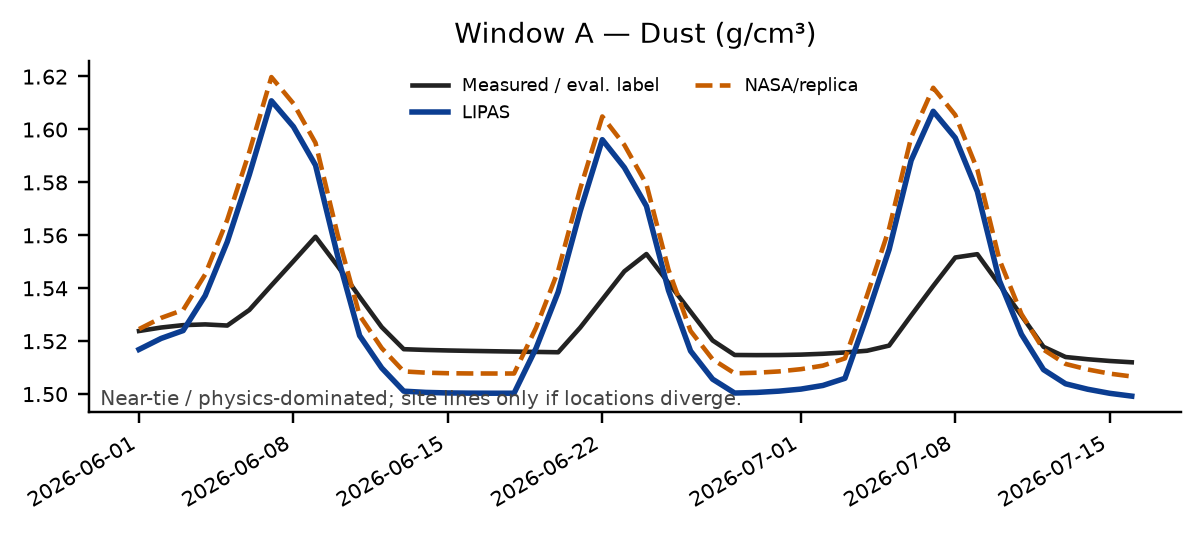
\includegraphics[width=\linewidth,height=0.18\textheight,keepaspectratio]{figures/fig_windowA_dust_g_cm3.png}
\captionof{figure}{Window A dust. Near-circular / physics-dominated; site lines for LIPAS and NASA.}
\label{fig:winAdust}
\end{minipage}
\end{center}

\begin{center}
\centering
\begin{tabular}{@{}lccc@{}}
\toprule
Hazard & Hybrid & Replica & Outcome \\
\midrule
Solar activity & 9.532 & 9.889 & Hybrid lower by about 3.6\% \\
Radiation (mSv) & 0.798 & 0.829 & Hybrid lower by about 3.7\% \\
Temperature ($^\circ$C) & 25.90 & 27.35 & Hybrid lower by about 5.3\% \\
Moonquakes / day & 1.166 & 1.167 & Hybrid residual lower \\
Micrometeorites & 0.015 & 0.643 & Circular / shower-term illustration \\
Dust (g\,cm$^{-3}$) & 0.445 & 0.445 & Near-circular / physics-dominated \\
\bottomrule
\end{tabular}
\captionof{table}{Window A RMSE, 1 June to 4 August 2026, summer/quiet--mixed, 195 site-days (R6c\_caution\_cap090).}
\label{tab:winA}
\end{center}

\begin{multicols}{2}
\subsubsection{Window B, disturbed / storm}

Window B covers 20 April to 20 May 2024 at the same three sites (93 site-days). Space-weather drivers are elevated relative to the quietest 2026 intervals. Hybrid RMSE is lower than the replica on all six hazards (6/6). Solar activity improves substantially (11.22 versus 13.79). Radiation improves strongly (0.071 versus 0.172). Temperature and moonquakes show residual gains (38.56 versus 40.35; 1.263 versus 1.269). Micrometeorites again reflect circular shower-label construction (0.012 versus 0.564). Dust shows a measured edge (0.147 versus 0.163) that remains physics-dominated / near-circular. Figures~\ref{fig:winBsolar}--\ref{fig:winBdust} show the same two-column per-hazard layout as Window~A. The mission simulation later injects one scripted storm for warning-time comparison only; it is not a substitute for this disturbed window.
\end{multicols}

\begin{center}
\centering
\begin{minipage}[t]{0.48\textwidth}
\centering
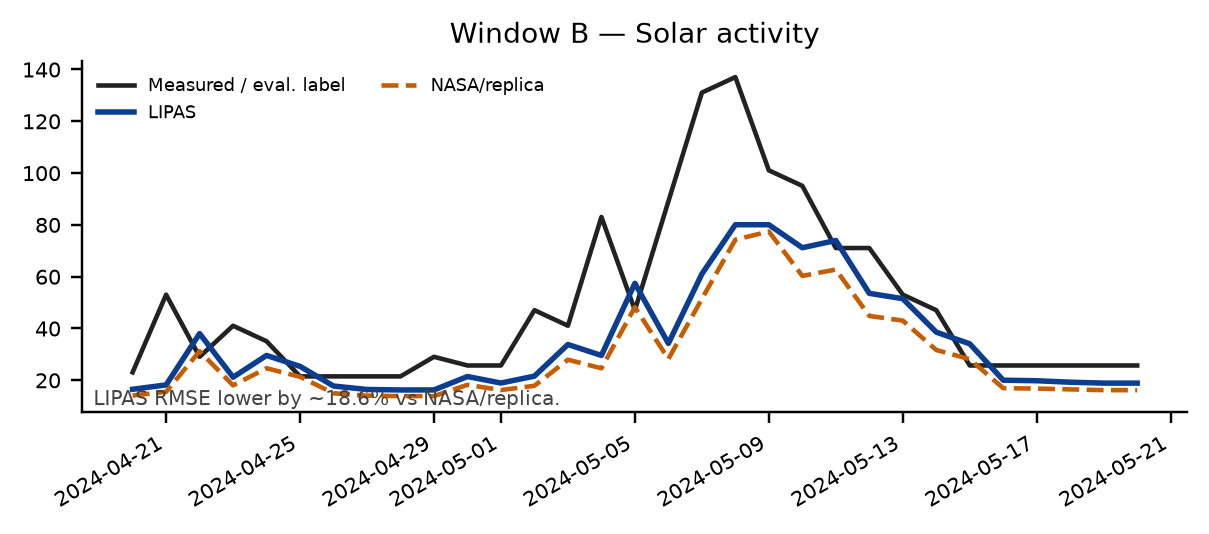
\includegraphics[width=\linewidth,height=0.18\textheight,keepaspectratio]{figures/fig_windowB_solar_activity.png}
\captionof{figure}{Window B solar. LIPAS RMSE $\sim$18.6\% lower than the NASA/replica.}
\label{fig:winBsolar}
\end{minipage}\hfill
\begin{minipage}[t]{0.48\textwidth}
\centering
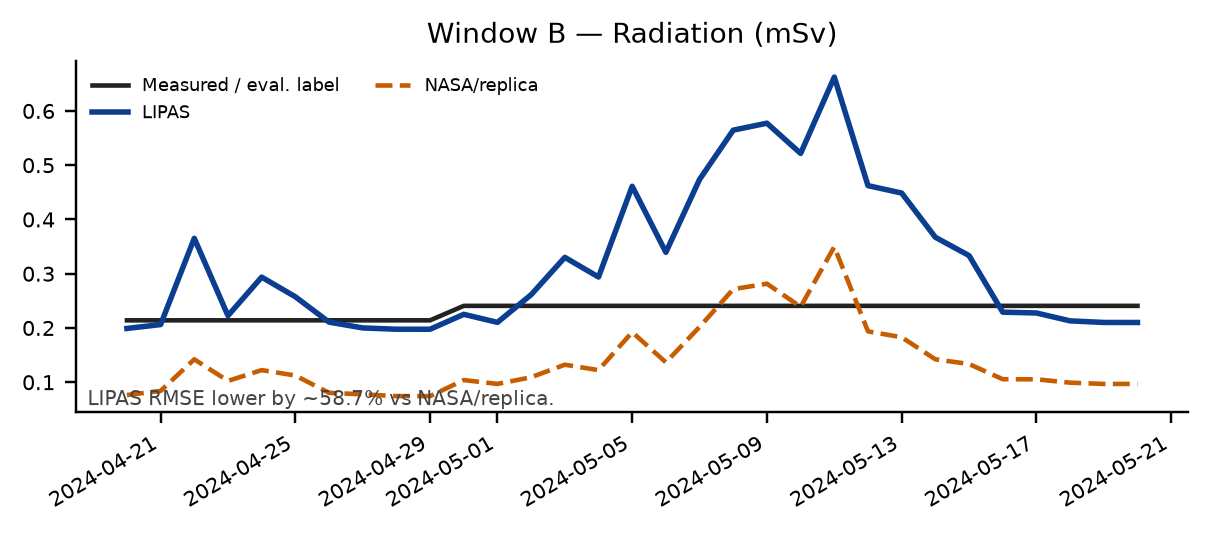
\includegraphics[width=\linewidth,height=0.18\textheight,keepaspectratio]{figures/fig_windowB_radiation_mSv.png}
\captionof{figure}{Window B radiation. LIPAS RMSE $\sim$58.7\% lower (ML share 0.15).}
\label{fig:winBrad}
\end{minipage}
\end{center}

\begin{center}
\centering
\begin{minipage}[t]{0.48\textwidth}
\centering
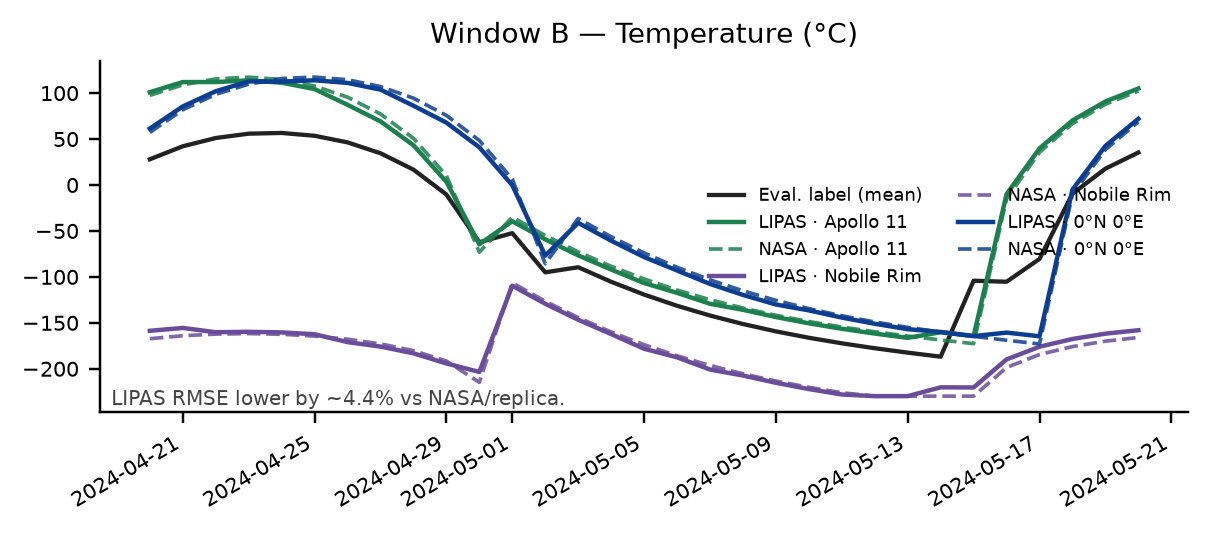
\includegraphics[width=\linewidth,height=0.18\textheight,keepaspectratio]{figures/fig_windowB_temperature_C.png}
\captionof{figure}{Window B temperature. LIPAS RMSE $\sim$4.4\% lower; site lines where locations diverge.}
\label{fig:winBtemp}
\end{minipage}\hfill
\begin{minipage}[t]{0.48\textwidth}
\centering
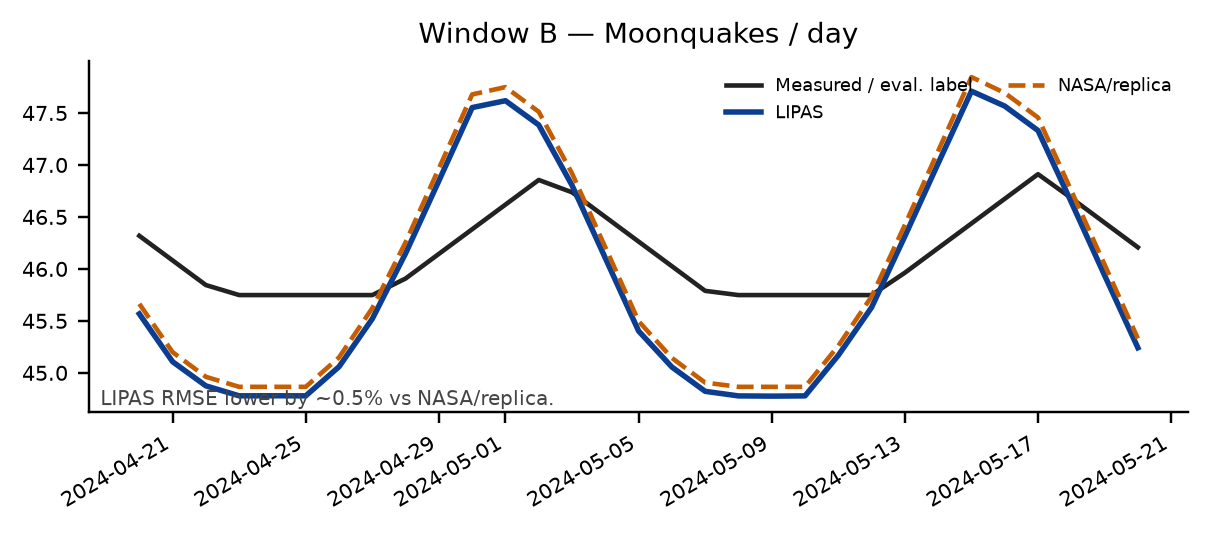
\includegraphics[width=\linewidth,height=0.18\textheight,keepaspectratio]{figures/fig_windowB_moonquakes_per_day.png}
\captionof{figure}{Window B moonquakes. Tiny residual edge; physics-dominated.}
\label{fig:winBmoon}
\end{minipage}
\end{center}

\begin{center}
\centering
\begin{minipage}[t]{0.48\textwidth}
\centering
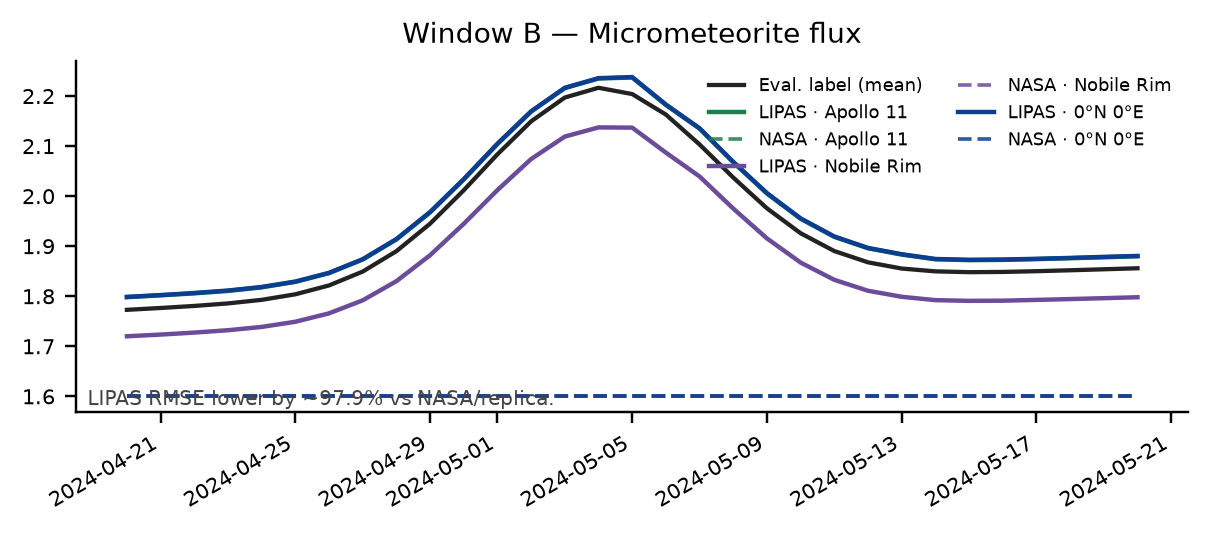
\includegraphics[width=\linewidth,height=0.18\textheight,keepaspectratio]{figures/fig_windowB_meteor_flux_1e15.png}
\captionof{figure}{Window B micrometeorites. Circular shower-label illustration, not an independent win.}
\label{fig:winBmeteor}
\end{minipage}\hfill
\begin{minipage}[t]{0.48\textwidth}
\centering
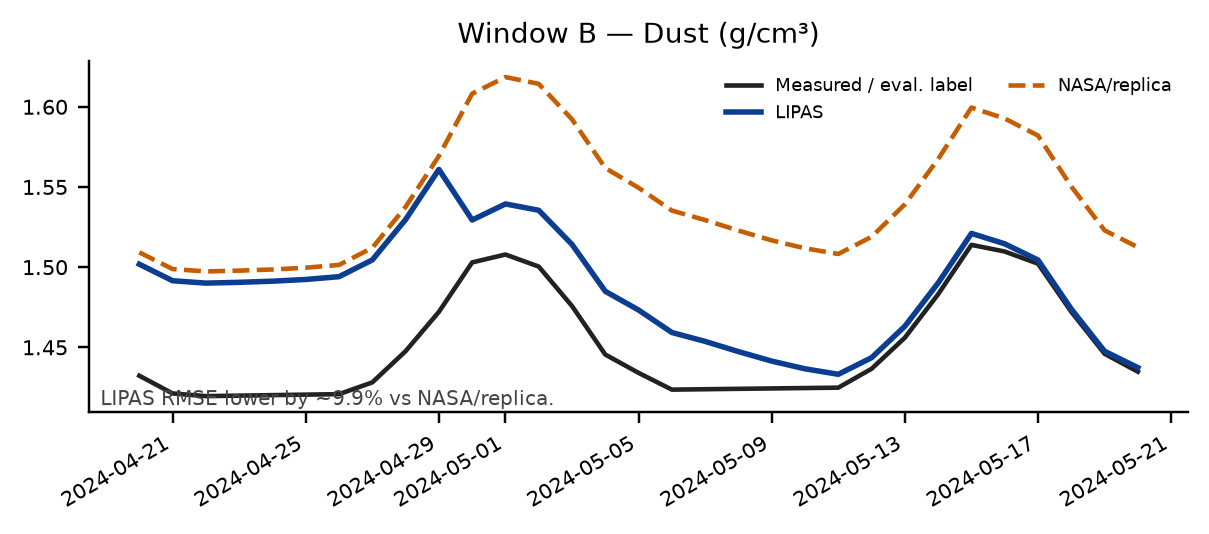
\includegraphics[width=\linewidth,height=0.18\textheight,keepaspectratio]{figures/fig_windowB_dust_g_cm3.png}
\captionof{figure}{Window B dust. Near-circular / physics-dominated; site lines for LIPAS and NASA.}
\label{fig:winBdust}
\end{minipage}
\end{center}

\begin{center}
\centering
\begin{tabular}{@{}lccc@{}}
\toprule
Hazard & Hybrid & Replica & Outcome \\
\midrule
Solar activity & 11.22 & 13.79 & Hybrid lower by about 18.6\% \\
Radiation (mSv) & 0.071 & 0.172 & Hybrid lower by about 58.7\% \\
Temperature ($^\circ$C) & 38.56 & 40.35 & Hybrid lower by about 4.4\% \\
Moonquakes / day & 1.263 & 1.269 & Hybrid residual lower \\
Micrometeorites & 0.012 & 0.564 & Circular / shower-term illustration \\
Dust (g\,cm$^{-3}$) & 0.147 & 0.163 & Near-circular / physics-dominated \\
\bottomrule
\end{tabular}
\captionof{table}{Window B RMSE, 20 April to 20 May 2024, disturbed/storm interval, 93 site-days (R6c\_caution\_cap090).}
\label{tab:winB}
\end{center}

\begin{multicols}{2}
\subsection{Operational mission simulation}

A radiation-focused EVA at the Apollo 11 site was simulated over 7 h 37 min, the duration of the second Apollo 17 EVA, to compare LIPAS warning times with those of separate public products under the R6c\_caution\_cap090 locked serve package. The same storm was injected on every path: a precursor at T+40, rising Kp and southward IMF Bz at T+55, and a GOES-like proton surge at T+70. Every path used the same thresholds, 0.095 mSv h$^{-1}$ for caution and 0.15 mSv h$^{-1}$ for no-go. The GOES-only path used proton flux alone, and the combined NASA path took the earlier of the proton warning and the geomagnetic or solar-driver warning.

Table~\ref{tab:mission} summarizes first caution and no-go times. LIPAS issued caution at T+50 and no-go at T+55. GOES alone reached caution at T+80 and no-go at T+105, and the combined path reached caution at T+55 and no-go at T+70. Relative to the proton surge at T+70, LIPAS caution occurred 20 minutes earlier. LIPAS no-go leads the GOES-only no-go by 50 minutes. The earlier LIPAS caution came from upstream solar and geomagnetic drivers, not from an event the proton product could not see. The exercise is radiation-focused. It does not show that LIPAS is safer on every hazard, and it does not replace an operator or flight-certified products.
\end{multicols}

\begin{center}
\centering
\begin{tabular}{@{}lcc@{}}
\toprule
System & First caution & First no-go \\
\midrule
LIPAS hybrid & T+50 min (0h 50m) & T+55 min (0h 55m) \\
NASA GOES proton product & T+80 min (1h 20m) & T+105 min (1h 45m) \\
NASA combined (physics rad + GOES) & T+55 min (0h 55m) & T+70 min (1h 10m) \\
\bottomrule
\end{tabular}
\captionof{table}{Mission-simulation caution and no-go times under the shared radiation-driven EVA script (R6c measured).}
\label{tab:mission}
\end{center}

\begin{center}
\centering
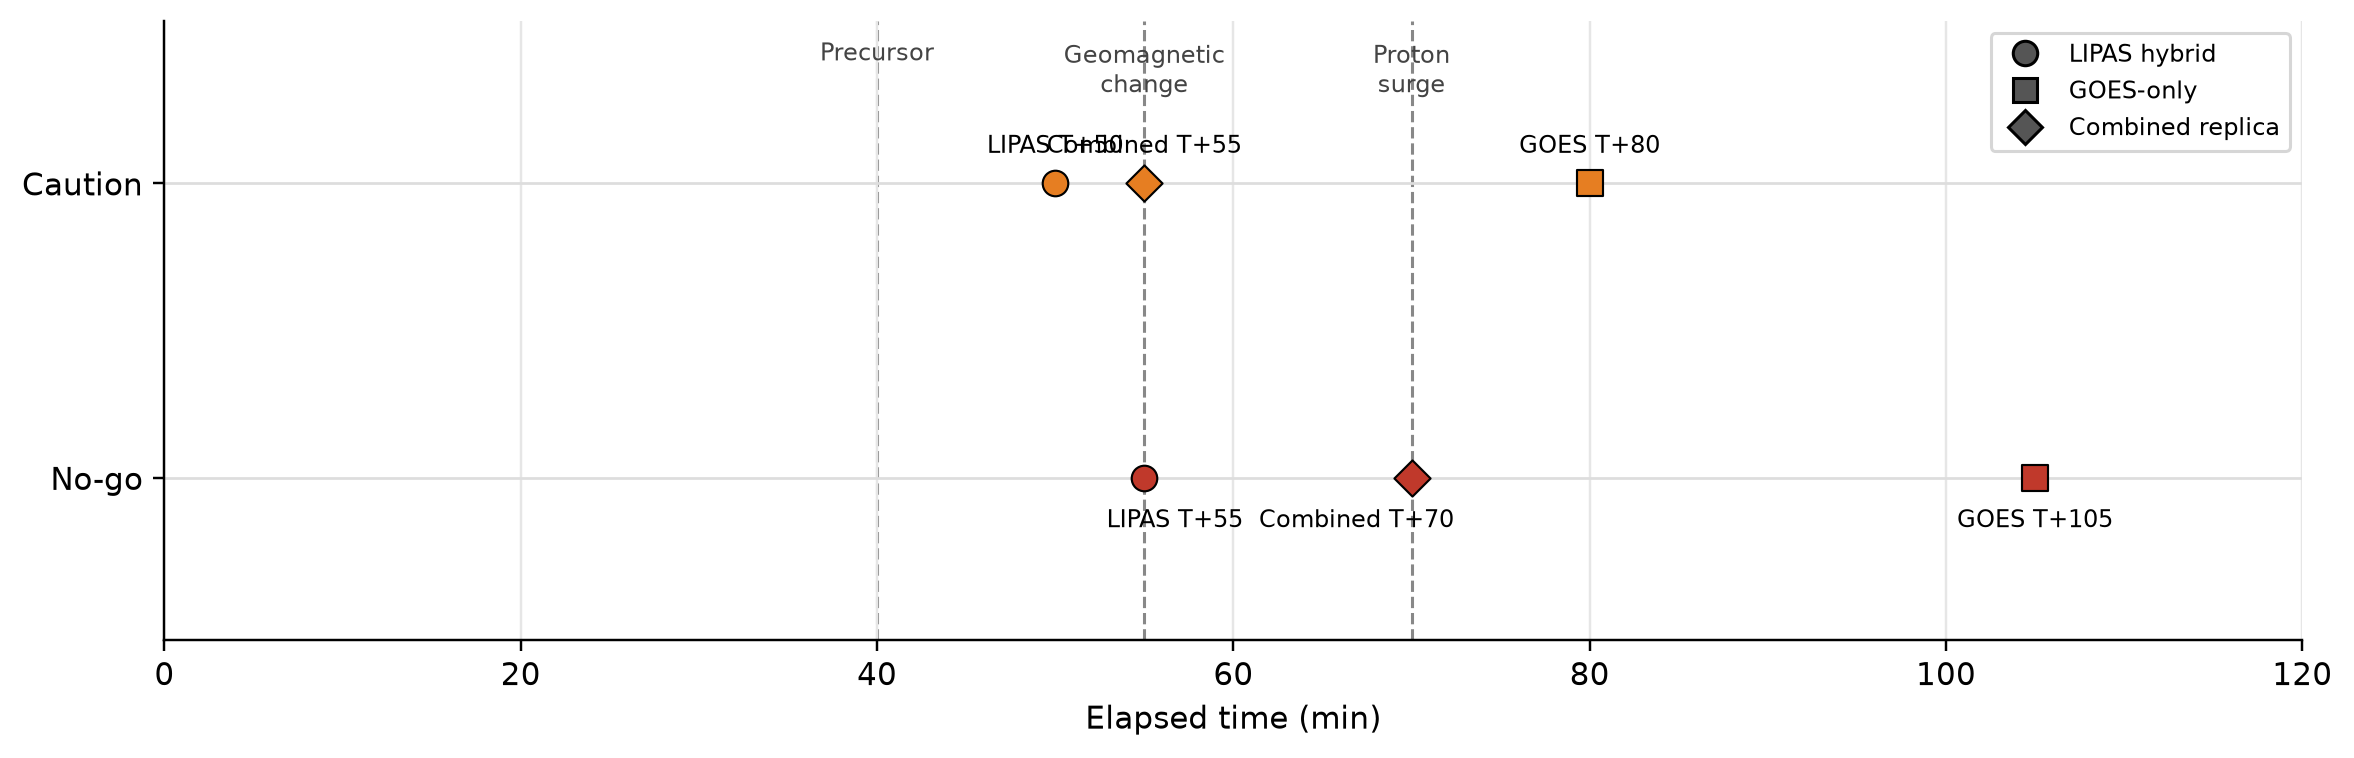
\includegraphics[width=\textwidth,height=0.26\textheight,keepaspectratio]{figures/fig_mission_timeline.png}
\captionof{figure}{Mission-simulation caution and no-go timeline (R6c measured): LIPAS, GOES-only, and combined replica, with precursor (T+40), geomagnetic change (T+55), and proton surge (T+70). Same events as Table~\ref{tab:mission}.}
\label{fig:mission}
\end{center}

\begin{multicols}{2}
\subsection{Input ablation}

The ablation study keeps the locked R6c\_caution\_cap090 serve package fixed and uses the quiet 17--30 June 2026 fortnight inside Window~A (42 site-days). One input at a time, and selected input pairs, are replaced with their Window~A means; the model is not retrained. Tables~\ref{tab:ablation-rad} and~\ref{tab:ablation-solar} report the resulting RMSE values. In the full-minus-case column, a negative value means that the altered configuration had a higher error than the full model. Baseline full-model RMSE is 1.702 on radiation and 11.56 on solar activity. On both channels, the worst one-away case is replacing the live solar input: radiation rises from 1.702 to 1.706 (about 0.23\%), and solar rises from 11.56 to 12.81 (about 10.7\%). Other single replacements leave both channels nearly unchanged. Section 6 discusses possible explanations.
\end{multicols}

\begin{center}
\centering
\begin{tabular}{@{}lccc@{}}
\toprule
Configuration & RMSE & Full minus case & Relative change \\
\midrule
Full model & 1.702 & 0.000 & 0.0\% \\
Set solar to mean & 1.706 & $-0.004$ & $-0.23\%$ \\
Set solar and temperature to mean & 1.706 & $-0.004$ & $-0.23\%$ \\
Set dust to mean & 1.702 & ${\sim}0$ & ${\sim}0\%$ \\
Set micrometeorites to mean & 1.702 & ${\sim}0$ & ${\sim}0\%$ \\
Set temperature to mean & 1.702 & ${\sim}0$ & ${\sim}0\%$ \\
Set moonquakes to mean & 1.702 & ${\sim}0$ & ${\sim}0\%$ \\
Set radiation to mean & 1.700 & $+0.002$ & $+0.11\%$ \\
\bottomrule
\end{tabular}
\captionof{table}{Radiation-channel sensitivity results from R6c input ablation (17--30 June 2026). Changes are full-model RMSE minus configuration RMSE.}
\label{tab:ablation-rad}
\end{center}

\begin{center}
\centering
\begin{tabular}{@{}lccc@{}}
\toprule
Configuration & RMSE & Full minus case & Relative change \\
\midrule
Full model & 11.56 & 0.00 & 0.0\% \\
Set solar to mean & 12.81 & $-1.24$ & $-10.7\%$ \\
Set solar and micrometeorites to mean & 12.80 & $-1.24$ & $-10.7\%$ \\
Set radiation to mean & 11.58 & $-0.02$ & $-0.17\%$ \\
Set micrometeorites to mean & 11.56 & ${\sim}0$ & ${\sim}0\%$ \\
Set temperature to mean & 11.56 & ${\sim}0$ & ${\sim}0\%$ \\
Set dust to mean & 11.56 & ${\sim}0$ & ${\sim}0\%$ \\
Set moonquakes to mean & 11.56 & ${\sim}0$ & ${\sim}0\%$ \\
\bottomrule
\end{tabular}
\captionof{table}{Solar-activity sensitivity results from R6c input ablation (17--30 June 2026). Changes are full-model RMSE minus configuration RMSE.}
\label{tab:ablation-solar}
\end{center}
\section{Discussion}
\begin{multicols}{2}
The studies reported in Section 5 show that the usefulness of machine learning, physics-based modelling and data integration in LIPAS depends on the hazard being forecast and on the purpose for which the output is used. This section interprets those results, sets out what they do and do not show, and identifies the limitations that bound the answers to the research questions given in Section 8. Combining physics and machine learning is not itself new (Karpatne et al., 2017; Willard et al., 2022; Camporeale, 2019). Theory-guided and physics-informed approaches have already been applied across environmental and space-weather problems. The contribution of LIPAS is narrower: the application of hazard-specific weighting, uncertainty-aware blending and cross-hazard inputs within a single lunar forecasting and decision-support system. In LIPAS the Python physics-estimation function supplies a physically grounded value for each hazard, the learned correction from the LSTM trunk is blended with it through Eqs. (2) and (3), and public heliophysics data enter as inputs to both paths rather than as a third modelling method. The results provide preliminary support for this design, while also showing that the architecture should not be treated as a replacement for specialised scientific models or as a fully validated operational forecasting system. The development record is important for interpreting the final architecture, and it must be read separately from the quantitative evidence. The April diagnostics used the browser prototype, not the locked hybrid model, and compared it with weakly replicated baselines at a single daytime site. That weak-replica setup is why early multi-hazard ``wins'' are diagnostic rather than locked-model skill, and its scores are not pooled with the locked-model results. Its actionable finding was the off-chart runaway of physically constrained channels alongside the temperature miss against the Diviner-style dayside relation, which motivated the migration to a server-assisted backend and the decision to keep temperature, moonquakes, micrometeorites and dust on the physics path. Every quantitative claim in Windows A and B, the mission simulation and the ablation therefore rests on the locked production model from the second training run, served under the R6c\_caution\_cap090 blend and archive-prior package. The locked serve blend weights are [0.40, 0.15, 0.02, 0.02, 0.03, 0.01] for solar activity, radiation, temperature, moonquakes, micrometeorites and dust, with storm-aware adaptive gating retained. Overnight LSTM ladder runs (T4a/b/c) did not beat the train-2 chronological held-out RMSE of about 4.97, so the LSTM weights remain train-2; R6c is a serve/physics/archive promote on those weights (R5s2 plus caution\_cap090). Temperature and moonquakes show residual hybrid gains rather than exact physics ties. Dust remains physics-dominated and near-circular: hybrid--physics correlation is essentially one, and the measured edge should not be read as independent dust sensing. Micrometeorite evaluation labels are shower-augmented physics (circular construction), so large replica gaps illustrate shower timing rather than independent forecast skill. More generally, much of the data and many of the approaches used to build the comparison targets overlap with those used to build LIPAS itself. Where that overlap is large, agreement between LIPAS and its references partly measures internal consistency rather than predictive accuracy. This is also why the uncertainty-guided weighting matters. LIPAS does not simply average a machine-learning prediction with a physics estimate. Within each channel's locked base weight, Eq. (3) reduces the learned contribution when the Monte Carlo dropout spread widens, shifting the forecast toward the physics path when the network is less certain. The purpose of the architecture was not to force machine learning into every channel, but to allow different sources of information to carry different levels of influence. Solar activity remains the channel with the largest learned weight (0.40). Hybrid RMSE is lower than the replica in summer Window A (9.532 versus 9.889) and in disturbed Window B (11.22 versus 13.79). Radiation improves in both locked windows (0.798 versus 0.829 in A; 0.071 versus 0.172 in B) with ML share 0.15. Gains rest on two locked windows at three sites (195 site-days in A; 93 in B). The micrometeorite results need careful reading. The physics path combines the MEM 3 export with AMS-based shower modulation, and the evaluation series carries the same shower family, so the large RMSE gaps (0.015 versus 0.643 in A; 0.012 versus 0.564 in B) are circular illustrations of shower timing rather than independent forecast wins. They do not demonstrate superiority over the complete NASA micrometeorite modelling framework, and they are not validated against measured lunar impact rates. The mission simulation shows why predictive performance and operational usefulness are not the same thing. In the radiation-focused EVA scenario, LIPAS issued caution at T+50, ten minutes after the injected precursor at T+40 and twenty minutes before the proton surge at T+70, and reached no-go at T+55. The GOES-only path reached caution at T+80 and no-go at T+105, while the combined NASA path reached caution at T+55 and the earlier hard no-go at T+70. LIPAS no-go therefore leads GOES-only no-go by fifty minutes. The earlier LIPAS caution came from upstream solar and geomagnetic drivers, not from an event that the proton product could not see. The result should not be interpreted as LIPAS detecting a storm that NASA could not detect. Instead, it shows that different pathways produce different warning times depending on which signals they monitor and how those signals are mapped to thresholds. The scenario used a single injected storm, predefined caution and no-go thresholds, and one hazard. It did not measure usability with mission personnel, it does not show that LIPAS is safer on every hazard, and it is not a proof of operational safety. A unified system can also concentrate risk if its data feeds or service fail, which a set of independent products partly avoids.

The ablation study provides evidence of cross-hazard sensitivity inside the locked model, but not of causation. It used a quiet Window~A fortnight (17--30 June 2026) and replaced one input at a time with its Window~A mean, without retraining. On both radiation and solar channels, replacing the solar input was the worst one-away case: radiation rose from 1.702 to 1.706 (about 0.23\%), and solar rose from 11.56 to 12.81 (about 10.7\%), while other single replacements left both channels nearly unchanged. The ablation measures how far the output moves when one input is held at its average; it does not show that one hazard causes another. Looking across the full set of results, different hazards benefit from different forms of information. Solar and radiation show clear hybrid gains under the R6c blend, especially in the storm window. Temperature and moonquakes show residual gains. Dust remains near-circular / physics-dominated. Micrometeorite behaviour is determined by explicit shower timing and circular labels rather than by independent machine-learning skill. LIPAS therefore does not behave as six identical machine-learning models; it acts as a framework that assigns different levels of influence to different sources of information depending on the hazard. Several limitations affect the strength of these conclusions. First, continuous co-located lunar-surface measurements do not exist for all six hazards, so quantitative targets are evaluation labels constructed from public observations, physical formulations, historical catalogs and proxies. The results describe comparative behaviour within this evaluation framework, not accuracy against complete lunar-surface truth. Second, except for the available MEM 3 engineering-model export, the comparisons are replicas: author-built reconstructions of publicly documented methods and data, not executions of agency operational software. Their value is methodological comparability under shared inputs, dates and locations, and they should not be read as runs of the agencies' own systems. Third, the qualitative comparison in Section 5.2 is a criteria matrix, not a ranking, and it does not say that LIPAS is more accurate than any specialist archive or model. Fourth, the quantitative evidence covers two locked windows, three sites and one locked serve package on train-2 LSTM weights; Window A is summer/quiet--mixed and Window B is the disturbed April--May 2024 interval. The strongest conclusion is therefore not that LIPAS replaces specialised NASA or NOAA models. Its value lies in providing a common forecasting and decision-support layer in which established physics, public heliophysics inputs, cross-hazard relationships and uncertainty estimates can be considered together. The results support this concept as a promising direction, while showing that substantial validation is still required before operational use.
\end{multicols}
\section{Future work}
\begin{multicols}{2}
LIPAS already provides a multi-hazard decision-support system for lunar operations, but further work is needed before it can be considered a trusted operational forecasting tool. The locked evaluation windows, mission simulation and ablation study have clarified where that work should focus. Rather than repeating the evaluations already completed, future work should build directly on their findings.

\subsection{Radiation and storm-window solar}

Radiation now shows hybrid gains in both locked windows under ML share 0.15, including a large storm-window margin, so the priority shifts to hardening those gains across additional disturbed periods and clarifying which component of the radiation path carries the skill. Storm-window solar now clears the replica (11.22 versus 13.79) and should still be tested with denser OMNI, DONKI and SWPC sampling, improved treatment of proton-flux events, and calibrated uncertainty estimates for radiation alerts. Differences between LIPAS and the combined NASA warning path should be examined transparently rather than resolved by retrospective threshold tuning.

\subsection{Solar input behaviour}

The solar ablation result deserves closer investigation. Under the R6c quiet fortnight, replacing the live solar input raised solar RMSE by about 10.7\%. Repeating the ablation under stronger solar activity, and with retrained rather than mean-substituted configurations, would show when the live solar input provides the greatest benefit. The solar gains should also be tested over longer periods and additional sites.

\subsection{Physics-tied channels and independent labels}

Temperature and moonquakes now carry small residuals, but dust and micrometeorites remain physics-dominated with circular or near-circular evaluation risk. Future work should obtain targets independent of the physics path, strengthen meteor-shower timing and MEM 3 integration, and score micrometeorites against observations that do not already contain the LIPAS shower term, so that those channels can be assessed rather than only illustrated.

\subsection{Validation with measured data}

As data become available from Artemis missions, lunar landers, rovers and orbital instruments, evaluation labels should be replaced with direct measurements wherever possible. Where measurements are not yet available, estimated labels should continue to be identified clearly. Collaboration with NASA, NOAA, ESA, JAXA and university research groups would strengthen validation through access to additional datasets, operational expertise and missionrelevant performance criteria.

\subsection{Operational development}

Future development of the LIPAS interface and mission planner should improve uncertainty visualisation, mission-specific alert thresholds and reports aligned with existing operational checklists. Mission simulations should extend beyond a single radiation storm to multi-hazard scenarios, should test behaviour when data feeds fail, and should measure usability with mission personnel. Interface improvements are valuable only if they communicate the underlying scientific results accurately and transparently.

\subsection{Extending the framework beyond the lunar surface}

Because much of the system already relies on heliophysics data, extending the framework to cislunar space and Earth orbit is a logical next step, with Mars as a longerterm possibility. These environments offer substantially more observational data than the lunar surface, allowing more rigorous validation of the hybrid method. The multi-hazard architecture and channelspecific weighting could be reused without a complete redesign. The immediate priorities are therefore to harden radiation and storm-window solar behaviour, explain the quiet-window solar ablation result, and obtain independent evaluation labels for micrometeorites and dust. Over the medium term, measured data and collaboration with space agencies should improve confidence in the system. Throughout its development, LIPAS should remain a consultative decision-support platform designed for incomplete observations, used alongside NASA and NOAA products rather than as a replacement for specialised scientific models or flightqualified systems.
\end{multicols}
\section{Conclusion}
\begin{multicols}{2}
This research examined whether machine learning can be integrated into a unified, physics-based lunar forecasting system while retaining the physical foundations of established environmental models. Regarding the first research question, a hybrid lunarforecasting system can be developed by combining machine-learning and physics-based approaches. The development process showed that a hazard-specific blend was more appropriate than applying machine learning uniformly: the prototype diagnostics exposed instability in physically constrained channels, which led to a locked hybrid on train-2 LSTM weights with R6c\_caution\_cap090 serve blend [0.40, 0.15, 0.02, 0.02, 0.03, 0.01]. Later overnight LSTM ladders did not beat the train-2 held-out RMSE, so the promote is serve/physics/archive rather than a new LSTM. The second research question asked whether integrating multiple hazards and data sources into one decision-support system can support operational decision-making alongside existing public products. The radiation-focused mission simulation answered it partially: LIPAS issued caution at T+50 and no-go at T+55, earlier than the GOES-only path (T+80 / T+105) because it drew on upstream solar and geomagnetic drivers, but the combined NASA path reached the hard no-go first at T+70, and the study did not establish that LIPAS is safer than existing approaches. The third research question asked whether the locked hybrid improves prediction performance relative to replicated public baselines and physics-only references. Under R6c, Window A and Window B both meet 6/6. Solar and radiation show hybrid gains in both windows, with the largest margins in the storm window; temperature and moonquakes show residual gains; micrometeorites remain circular shower-label illustrations; and dust remains near-circular / physics-dominated. The principal contribution of LIPAS is therefore not the replacement of existing lunar models but their integration into a single forecasting and decision-support framework. The studies show both where a constrained hybrid architecture can add predictive value and where honesty limits still apply, and they define the validation that must follow before LIPAS can support lunar operations alongside NASA and NOAA products.

\section*{Acknowledgements}

The author thanks Benjamin Irani-Fey for coding support during the NASA Space Apps Challenge. The author also thanks NASA, NOAA, and other space agencies and research organizations for the public lunar-mission data and space-weather archives that made the project possible, and thanks Polygence research mentor Kyle Kennedy for support in redesigning and reevaluating the studies, methods, and conclusions.

\subsection*{CRediT author statement}
Luka Takki: Conceptualization, Methodology, Software, Validation, Formal analysis, Investigation, Data curation, Visualization, Writing: original draft, and Writing: review and editing.

\subsection*{Funding}
This research received no specific grant from funding agencies in the public, commercial, or not-for-profit sectors.

\subsection*{Declaration of competing interest}
The author declares that there are no known competing financial interests or personal relationships that could have appeared to influence the work reported in this paper.

\subsection*{Data and code availability}
Public sources are listed in the references; numerical tables accompany the paper. Dashboard: \url{https://lipas.netlify.app}. Code and locked model weights: \url{https://github.com/Luka-bot-afk/LIPAS} (numerical tables and \texttt{locked\_saved\_model} in the papers/appendix\_numerical\_tables folder).

\section*{Declaration of generative AI and AI-assisted technologies in the manuscript preparation process}

During the preparation of this work, the author used Cursor and Google Gemini to review, and to help modify, selected parts of the code and the manuscript. These tools did not write the paper. The author checked every suggested change, made the final edits, and takes full responsibility for the content of the published article. Their role was limited to review and selective modification of existing material; they were not used to draft or author the manuscript. 

\section*{References}

\subsection*{Literature overview and hybrid methods}
Camporeale, E., 2019. The challenge of machine learning in space weather: Nowcasting and forecasting. Space Weather 17, 1166--1207. doi:10.1029/2018SW002061.

Hochreiter, S., Schmidhuber, J., 1997. Long short-term memory. Neural Computation 9, 1735--1780. doi:10.1162/neco.1997.9.8.1735.

Karpatne, A., et al., 2017. Theory-guided data science: A new paradigm for scientific discovery from data. IEEE Transactions on Knowledge and Data Engineering 29, 2318--2331. doi:10.1109/TKDE.2017.2720168.

Willard, J., Jia, X., Xu, S., Steinbach, M., Kumar, V., 2022. Integrating scientific knowledge with machine learning for engineering and environmental systems. ACM Computing Surveys 55, 1--37. doi:10.1145/3514228.

Cucinotta, F.A., Hu, S., Schwadron, N.A., Kozarev, K., Townsend, L.W., Kim, M.H.Y., 2010. Space radiation risk limits and earth-moon-mars environmental models. Space Weather 8, S00E09. doi:10.1029/2010SW000572.

Hassler, D.M., et al., 2014. Mars' surface radiation environment measured with the mars science laboratory's curiosity rover. Science 343, 1244797. doi:10.1126/science.1244797.

Minow, J.I., et al., 2020. Space Weather Architecture Options to Support Human and Robotic Deep Space Exploration. Technical Report NASA/TM-20205000837. NASA. URL: \url{https://ntrs.nasa.gov/citations/20205000837}.

Zeitlin, C., et al., 2013. Measurements of energetic particle radiation in transit to mars on the mars science laboratory. Science 340, 1080--1084. doi:10.1126/science.1235989.

\subsection*{Lunar hazard models and archives}
Colwell, J.E., Batiste, S., Horanyi, M., Robertson, S., Sture, S., 2007. Lunar surface: Dust dynamics and regolith mechanics. Reviews of Geophysics 45, RG2006. doi:10.1029/2005RG000184.

Hayne, P.O., Williams, J.P., Bandfield, J.L., Vasavada, A.R., Greenhagen, B.T., Siegler, M.A., Paige, D.A., Tyler, G.L., 2017. Global regolith thermophysical properties of the moon from the lunar reconnaissance orbiter diviner radiometer. Journal of Geophysical Research: Planets 122, 2371--2400. doi:10.1002/2017JE005387.

Horanyi, M., Szalay, J.R., Kempf, S., Schmidt, J., Grun, E., Srama, R., Sternovsky, Z., 2015. A permanent, asymmetric dust cloud around the moon. Nature 522, 324--326. doi:10.1038/nature14479.

Kawamura, T., Tanaka, S., Saito, Y., Horleston, A.C., Charalambous, C., Lognonne, P., Banerdt, W.B., Team, A.S., 2017. Re-analysis of apollo seismic data and implications for deep moonquakes. Journal of Geophysical Research: Planets 122, 114--132. doi:10.1002/2016JE005230.

Lammlein, D.R., 1977. Lunar seismicity and tectonics. Physics of the Earth and Planetary Interiors 14, 224--273.

Langseth, M.G., Keihm, S.J., Peters, K., 1972. Revised lunar heat-flow values, in: Proceedings of the Third Lunar Science Conference, MIT Press. pp. 3143--3171.

Moorhead, A.V., Koehler, H.M., Cooke, W.J., 2020. NASA Meteoroid Engineering Model Release 3 (MEM 3). Technical Report. NASA. URL: \url{https://ntrs.nasa.gov/citations/20200001093}.

Nakamura, Y., 2005. Farside deep moonquakes and deep interior of the moon. Journal of Geophysical Research: Planets 110, E01001. doi:10.1029/2004JE002332.

Nunn, C., et al., 2020. Lunar seismology: A data and instrumentation review. Space Science Reviews 216, 89. doi:10.1007/s11214-020-00709-3.

Onodera, K., 2024. Reanalysis of apollo seismic data reveals 22,000 previously undetected moonquakes. Journal of Geophysical Research: Planets 129, e2023JE008153. doi:10.1029/2023JE008153.

Paige, D.A., et al., 2010. The lunar reconnaissance orbiter diviner lunar radiometer experiment. Space Science Reviews 150, 125--160. doi:10.1007/s11214-009-9529-2.

Schwadron, N.A., et al., 2014. Does the worsening galactic cosmic radiation environment observed by crater preclude future manned deep-space exploration? Space Weather 12, 622--632. doi:10.1002/2014SW001084.

Spence, H.E., et al., 2010. Crater: The cosmic ray telescope for the effects of radiation experiment on the lunar reconnaissance orbiter mission. Space Science Reviews 150, 243--284. doi:10.1007/s11214-009-9584-8.

Stubbs, T.J., Vondrak, R.R., Farrell, W.M., 2006. A dynamic fountain model for lunar dust. Advances in Space Research 37, 59--66. doi:10.1016/j.asr.2005.04.005.

Szalay, J.R., Horanyi, M., 2015. Annual variation and synodic modulation of the sporadic meteoroid flux to the moon. Geophysical Research Letters 42, 10580--10584. doi:10.1002/2015GL066898.

Vasavada, A.R., Paige, D.A., Wood, S.E., 1999. Near-surface temperatures on mercury and the moon and the stability of polar ice deposits. Icarus 141, 179--193. doi:10.1006/icar.1999.6175.

Williams, J.P., Paige, D.A., Greenhagen, B.T., Sefton-Nash, E., 2017. The global surface temperatures of the moon as measured by the diviner lunar radiometer experiment. Icarus.

\subsection*{Public data products and agency sources}
American Meteor Society, 2026. Meteor shower calendar. URL: \url{https://www.amsmeteors.org/meteor-showers/meteor-shower-calendar}.

International Meteor Organization, 2026. Meteor shower calendar resources. URL: \url{https://www.imo.net/resources/calendar}.

King, J.H., Papitashvili, N.E., 2005. Solar wind spatial scales in and comparisons of hourly wind and ace plasma and magnetic field data. Journal of Geophysical Research 110, A02104. doi:10.1029/2004JA010649.

NASA, 2020. NASA's lunar exploration program overview. URL: \url{https://www.nasa.gov/specials/artemis/}.

NASA, 2023a. Diviner lunar radiometer experiment data products. URL: \url{https://pds-geosciences.wustl.edu/lro/lro-l-dlre-4-rdr-v1.0/}.

NASA, 2023b. DONKI API documentation. URL: \url{https://api.nasa.gov/DONKI/}.

NASA, 2023c. LRO CRaTER data products. URL: \url{https://pds-geosciences.wustl.edu/missions/lro/crater.htm}.

NASA Goddard Space Flight Center, 2026. Space physics data facility OMNI database. URL: \url{https://omniweb.gsfc.nasa.gov}.

NASA Planetary Data System, 2015. LADEE LDEX calibrated data.

National Oceanic and Atmospheric Administration, 2023. Space weather prediction center datasets: GOES primary X-ray flux, integral protons, and planetary K-index. URL: \url{https://services.swpc.noaa.gov/}.

\subsection*{Software and tooling}
Cesium GS, 2026. CesiumJS 3D geospatial virtual globe engine. URL: \url{https://cesium.com}.

Chart.js Contributors, 2026. Chart.js open-source canvas graphing toolset. URL: \url{https://www.chartjs.org}.

Chollet, F., et al., 2015. Keras. URL: \url{https://keras.io/}.

Google TensorFlow Team, 2026. TensorFlow machine learning and deep learning ecosystem. URL: \url{https://www.tensorflow.org}.

The reported experiments are reproduced in the Supplementary Appendices. Code and study scripts: \url{https://github.com/Luka-bot-afk/LIPAS}. Daily tables and the locked model weights are in papers/appendix\_numerical\_tables/ (see the reproduction appendix).
\end{multicols}
\appendix
\onecolumn
\section*{Appendices}
\addcontentsline{toc}{section}{Appendices}
\section{Numerical tables}

The short RMSE tables for Windows A and B (R6c) are in \texttt{reported\_window\_rmse\_R6.md}. The daily rows remain in the numerical PDF for the prior draft lineage; if the preview is blank, the Download option opens the file. April rows start after the cover page. Window A covers 1 June--4 August 2026; Window B (storm) covers 20 April--20 May 2024.

\begin{itemize}
\item \url{https://github.com/Luka-bot-afk/LIPAS/blob/main/papers/appendix_numerical_tables/reported_window_rmse_R6.md}
\item \url{https://github.com/Luka-bot-afk/LIPAS/blob/main/papers/appendix_numerical_tables/LIPAS_appendix_numerical_tables_A_B_D_E.pdf}
\end{itemize}

\section{Qualitative comparison framework}

DONKI, Diviner, LDEX, Apollo PSE, MEM 3, GOES-18, and LIPAS are scored on the nine criteria. The labels run from None to Very High. Labels are not converted into numbers or summed. Scores can be compared with Table~\ref{tab:qual}. The file also lists the documents used for each score.

\url{https://github.com/Luka-bot-afk/LIPAS/blob/main/papers/appendix_numerical_tables/LIPAS_qualitative_comparison_framework.md}

\subsection*{The nine criteria}
Hazard coverage, fusion across hazards, forecast lead, spatial detail, real-time use, robustness, validation, usability, and openness.

\subsection*{Documents used}
\begin{itemize}
\item NASA DONKI API documentation, \url{https://api.nasa.gov/DONKI/}
\item NOAA SWPC data services, \url{https://services.swpc.noaa.gov/}
\item Paige et al. (2010), Space Science Reviews, Diviner.
\item Williams et al. (2017), Icarus, Diviner global temperatures.
\item Horanyi et al. (2015), Nature, lunar dust and LDEX.
\item Nakamura (2005), Journal of Geophysical Research, deep moonquakes.
\item Nunn et al. (2020), Space Science Reviews, lunar seismology.
\item Moorhead et al. (2020), NASA MEM 3 technical report.
\item Spence et al. (2010) and Schwadron et al. (2014), CRaTER.
\item King and Papitashvili (2005), OMNI solar-wind scales.
\end{itemize}

\section{How the numbers are compared}

\subsection*{Sites and windows}
Sites are $0^{\circ}$N $0^{\circ}$E (E), Apollo 11 (A), and Nobile Rim (N). Window A is 1 June to 4 August 2026 (195 site-days, summer/quiet--mixed). Window B is 20 April to 20 May 2024 (93 site-days, disturbed/storm). The hazards are solar activity, radiation, temperature, moonquakes, micrometeorites, and dust.

\subsection*{Line-chart evaluation}
Window figures plot the evaluation label, the LIPAS hybrid, and the NASA/replica on a shared time axis. Storm Window~B emphasises the solar and radiation channels; Window~A shows one line chart per hazard.

The R6c\_caution\_cap090 serve blend in this paper is solar 0.40, radiation 0.15, temperature 0.02, moonquakes 0.02, micrometeorites 0.03, and dust 0.01, with storm-aware adaptive gating as in Section 3.2, on unchanged train-2 LSTM weights.

\section{How to rerun each study}

Code, configuration, data-processing helpers, and evaluation scripts for the reported studies are in the public repository: \url{https://github.com/Luka-bot-afk/LIPAS}. Step-by-step commands for each study are collected in \texttt{REPRODUCTION.md}:

\url{https://github.com/Luka-bot-afk/LIPAS/blob/main/papers/appendix_numerical_tables/REPRODUCTION.md}

The train-2 TensorFlow weights remain in \texttt{papers/appendix\_numerical\_tables/locked\_saved\_model/}. The R6c\_caution\_cap090 serve/physics/archive package used for the reported Window A/B, mission, and ablation numbers is in \texttt{saved\_model\_R6c\_caution\_cap090/} (and \texttt{studies/draft30\_r6/}). Reproduce with that package's blend weights [0.40, 0.15, 0.02, 0.02, 0.03, 0.01] and adaptive gating. Expected RMSE values for each study are listed with the commands below.

\begin{enumerate}
\item \textbf{Qualitative comparison (Table~\ref{tab:qual}).} The framework file linked in Appendix B records the scoring rules for the seven systems; labels can be compared with Table~\ref{tab:qual}.
\item \textbf{April prototype (Figure~\ref{fig:proto}).} The numerical PDF contains the April rows. This daytime run at $0^{\circ}$N, $0^{\circ}$E is not the locked window evaluation. There is no separate script, and these rows do not belong in Table~\ref{tab:winA} or Table~\ref{tab:winB}.
\item \textbf{Window A (Table~\ref{tab:winA}, Figures~\ref{fig:winAsolar}--\ref{fig:winAdust}).} \texttt{python scripts/run\_14day\_flagship\_study.py --start 2026-06-01 --end 2026-08-04 --window-label A --out-dir logs/overnight\_improve/train4/studies\_R6c\_draft30/A --model-dir saved\_model\_R6c\_caution\_cap090 --csv data/ingested\_extended/extended\_training\_window\_B\_ready.csv}. Solar RMSE should be about 9.532 versus 9.889. Radiation should be about 0.798 versus 0.829.
\item \textbf{Window B storm (Table~\ref{tab:winB}, Figures~\ref{fig:winBsolar}--\ref{fig:winBrad}).} The same script, with start 2024-04-20, end 2024-05-20, and window label B\_storm. Solar RMSE should be about 11.22 versus 13.79. Radiation should be about 0.071 versus 0.172.
\item \textbf{Mission simulation (Table~\ref{tab:mission}, Figure~\ref{fig:mission}).} Use the R6c package; measured caution/no-go times are LIPAS T+50 / T+55 and GOES T+80 / T+105 (see \texttt{studies/draft30\_r6/mission\_sim/}).
\item \textbf{Ablation (Tables~\ref{tab:ablation-rad} and~\ref{tab:ablation-solar}).} Quiet fortnight 17--30 June 2026 inside Window~A. Full-model radiation RMSE about 1.702 and solar about 11.56; worst one-away for both channels is remove solar (radiation +0.23\%; solar +10.7\%).
\end{enumerate}

\section{Train, validation, and test splits}
\label{app:splits}

Table~\ref{tab:splits} records the chronological split used for the locked second training run. Counts come from the locked-model metadata. Dates are the common per-site range after ordering each of the twelve training sites by time. The six hazards share one multi-output split; there is no separate hazard-specific cut. Windows A and B are locked evaluation sets reported in the Results and are not part of this training split.

\begin{center}
\begin{tabular}{@{}llrr@{}}
\toprule
Partition & Dates & Rows & Share \\
\midrule
Training & 1 Jan 1969 -- 12 Apr 2009 & 176\,544 & $\approx$70\% \\
Validation & 13 Apr 2009 -- 28 Nov 2017 & 37\,824 & $\approx$15\% \\
Chronological test & 29 Nov 2017 -- 16 Jul 2026 & 37\,824 & $\approx$15\% \\
\midrule
Total & 1 Jan 1969 -- 16 Jul 2026 & 252\,192 & 100\% \\
\bottomrule
\end{tabular}
\captionof{table}{Chronological train, validation, and test split for the locked model (twelve sites; all six hazards).}
\label{tab:splits}
\end{center}

\begin{center}
\begin{tabular}{@{}lll@{}}
\toprule
Locked evaluation set & Dates & Size \\
\midrule
Window A & 1 Jun--4 Aug 2026 & 195 site-days \\
Window B (storm) & 20 Apr--20 May 2024 & 93 site-days \\
\bottomrule
\end{tabular}
\captionof{table}{Locked evaluation windows used in the Results.}
\label{tab:evalwindows}
\end{center}
